% VDE Template for EUSAR Papers
% Provided by Barbara Lang und Siegmar Lampe
% University of Bremen, January 2002
% English version by Jens Fischer
% German Aerospace Center (DLR), December 2005
% Additional modifications by Matthias Wei{\ss}
% FGAN, January 2009

%-----------------------------------------------------------------------------
% Type of publication
\documentclass[a4paper,10pt]{article}
%-----------------------------------------------------------------------------
% Other packets: Most packets may be downloaded from www.dante.de and
% "tcilatex.tex" can be found at (December 2005):
% http://www.mackichan.com/techtalk/v30/UsingFloat.htm
% Not all packets are necessarily needed:
\usepackage[T1]{fontenc}
\usepackage[latin1]{inputenc}
%\usepackage{ngerman} % in german language if required
\usepackage[nooneline,bf]{caption} % Figure descriptions from left margin
\usepackage{times}
\usepackage{multicol}
\usepackage{amsmath}
\usepackage{amssymb}
\usepackage[dvips]{graphicx}
\usepackage{epsfig}
\usepackage{url}
\usepackage{framed}

\input{tcilatex}
%-----------------------------------------------------------------------------
% Page Setup
\textheight24cm \textwidth17cm \columnsep6mm
\oddsidemargin-5mm                 % depending on print drivers!
\evensidemargin-5mm                % required margin size: 2cm
\headheight0cm \headsep0cm \topmargin0cm \parindent0cm
\pagestyle{empty}                  % delete footer and header
%----------------------------------------------------------------------------
% Environment definitions
\newenvironment*{mytitle}{\begin{LARGE}\bf}{\end{LARGE}\\}%
\newenvironment*{mysubtitle}{\bf}{\\[1.5ex]}%
\newenvironment*{myabstract}{\begin{Large}\bf}{\end{Large}\\[2.5ex]}%
%-----------------------------------------------------------------------------
% Using Pictures and tables:
% - Instead "table" write "tablehere" without parameters
% - Instead "figure" write "figurehere " without parameters
% - Please insert a blank line before and after \begin{figuerhere} ... \end{figurehere}
%
% CAUTION:   The first reference to a figure/table in the text should be formatted fat.
%
\makeatletter
\newenvironment{tablehere}{\def\@captype{table}}{}
\newenvironment{figurehere}{\def\@captype{figure}\vspace{2ex}}{\vspace{2ex}}
\newcounter{CLCounter}
\newenvironment{CLCode}
{%
	\footnotesize\begin{framed}%
    \refstepcounter{CLCounter}%
  \textbf{OpenCL Reference (\arabic{CLCounter})\\}%
  \quad
}
{%
\end{framed}%
}
\makeatother



%%%%%%%%%%%%%%%%%%%%%%%%%%%%%%%%%%%%%%%%%%%%%%%%%%%%%%%%%%%%%%%%%%%%%%%%%%%%%%
\begin{document}
\nocite{*}
% Please use capital letters in the beginning of important words as for example
\begin{mytitle}INTRODUCTION TO OPENCL AND DEVICE FISSION\end{mytitle}
\begin{mysubtitle}\end{mysubtitle}
%
% Please do not insert a line here
%
\\
Arnaboldi Gabriele\\
Matr. 765568, (arnaboldi@libero.it)\\
\hspace{10ex}
\begin{flushright}
\emph{Report for the master course of Embedded Systems}\\
\emph{Reviser: PhD. Patrick Bellasi (bellasi@elet.polimi.it)}
\end{flushright}

Received: April, 01 2011\\
\hspace{10ex}

\begin{myabstract} Abstract \end{myabstract}
This is a normal text in 10pt type size and 12pt line spacing.
Place here a summary of your report. Focus on what is the problem and how you
propose to tackle it. Briefly resume achieved results.

Lorem ipsum dolor sit amet, consectetur adipiscing elit. Cras dapibus. Donec
fermentum mauris non lectus. Nulla porttitor pede id ante. Donec in erat
pellentesque erat ultrices rutrum. Pellentesque id tellus. Donec vel mi non dui
adipiscing tempor.  Nunc laoreet pede ut lectus. Aenean aliquam quam a sem. Duis
at elit? Ut dolor massa, dictum vel; convallis quis, ullamcorper id, urna.

\vspace{4ex}	% Please do not remove or reduce this space here.
\begin{multicols}{2}

%%%%%%%%%%%%%%%%%%%%%%%%%%%%%%%%%%%%%%%%%%%%%%%%%%%%%%%%%%%%%%%%%%%%%%%%%%%%%

%%%%%%%%%%%%%%%%%%%%%%%%%%%%%%%%%%%%%%%%%%%%%%%%%%%%%%%%%%%%%%%%%%%%%%%%%%%%%
\section{GPGPU Introduction}

GPGPU (\textit{General Purpose computation on Graphics Processor Unit}), also known as \textit{GPU Computing}, is the utilization of the graphic adapter of a personal computer to perform generic and non-graphic related computation usually handled by the CPU.\\
Once designed and optimized specifically to perform only graphic calculations, modern GPUs are evolving into \emph{high-performances many-core} processors that can be virtually used to perform any task, and developers who port their applications to GPUs are able to achieve speedups of orders of magnitude vs. optimized CPU implementations.\cite{GPGPUORG:About}\\
The reason why GPUs are so fast has to be searched [.... ... ] GPUs were born to deal with [extensive performace request by videogame]
Ottimizzate per fare poche e semplici operazioni su vertici e matrici, ma in PARALLELO -> parallelismo intriseco.
GPUs have been built to exploit application parallelism, and a single graphic adapter can host hundreds, if not thousands, of cores; this translates in TeraFlops of operations per second vs. the few GigaFlops a CPU can handle alone.//
 (incremento pi� alto di legge di moore?)

\begin{figurehere}
 \centering
 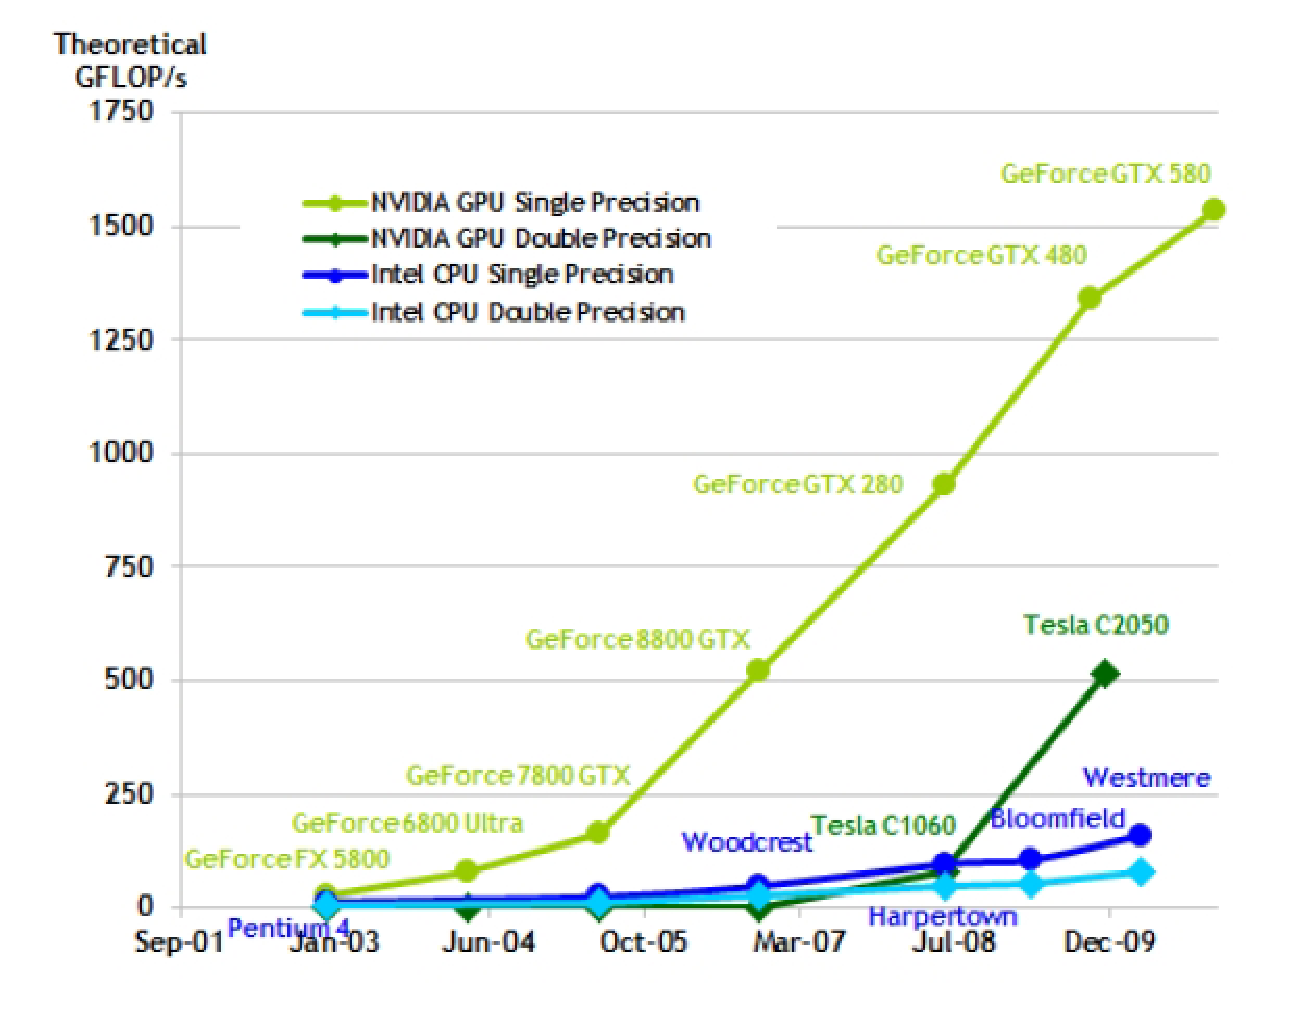
\includegraphics[width=8cm, height=4cm]{./eps/GPU_CPU_chart.eps}
 \caption{CPU vs GPU growth rate.}
 \label{fig:cpuvsgpu}
\end{figurehere}


-esempi applicativi
Due to its parallel nature, GPU computing can be very effective for applications involving huge amount of data, especially if the data can be structured in structures like vectors and arrays.
Parallel GPU computation can be applied in various applications and research-field, from computer vision, to mathematical simulations, to bio-informatics, often allowing to achieve in few months results that would have required years with a standard CPU-only approach (with speedups of even 250x,350x).

METTERE GRAFICO DEL PAPER??

As seen in TAB, GPU can offload the CPU from most of its work, but this doesn't mean that CPU performance is no longer critical. Many applications don't (and can't) map all their code to the GPU, and in certain cases the CPU can run some part of the code more effectively than the GPU.
Furthermore, not all the code can be mapped easily and clearly on the GPU, as programming in this say can be way more difficult than programming in a standard way, it is not possible to simply "`port"' the code from the CPU to the GPU.
-problemi: difficolt�

%-----------------------------------------------------------------------------
\subsection{Basic Principles}
% Please avoid separations in titles
% and separate text manually

In this section we'll analyze some of the basic principles behind GPGPU programming. Some of these concepts are directly related to and help to understand why GPU computing is so fast, for instance, GPUs can handle bidimensional matrices natively, while CPUs are limited to single dimension array.

\begin{itemize}
	\item Array \= Texture
	\item Kernels
	\item Feedback
	\item ....
\end{itemize}


%This is a citation \cite{Norman09Learn} and here is another citation
%\cite{Peyton93Howto}.  Lorem ipsum dolor sit amet, consectetur adipiscing elit.


%And this is the reference to a single column figure (see {\bf Figure
%\ref{fig:myfigure1}}).  Lorem ipsum dolor sit amet, consectetur adipiscing elit.

\begin{figurehere}
 \centering
 \includegraphics[width=8cm, height=4cm]{./eps/placeholder.eps}
 \caption{Some single-column figure caption.}
 \label{fig:myfigure1}
\end{figurehere}


%-----------------------------------------------------------------------------
\subsection{GPGPU Programming Languages}


\begin{figure*}[t]
  \centering
 \includegraphics[width=16cm, height=4cm]{./eps/placeholder.eps}
 \caption{Some wide-figure caption.}
 \label{fig:myfigure2}
\end{figure*}

And this is the reference to a single column figure (see {\bf Figure
\ref{fig:myfigure2}}). Lorem ipsum dolor sit amet, consectetur adipiscing elit.

%%%%%%%%%%%%%%%%%%%%%%%%%%%%%%%%%%%%%%%%%%%%%%%%%%%%%%%%%%%%%%%%%%%%%%%%%%%%%
%%%%%%%%%%%%%%%%%%%%%%%%%%%%%%%%%%%%%%%%%%%%%%%%%%%%%%%%%%%%%%%%%%%%%%%%%%%%%
\section{OpenCL and Device Fission} \label{sect:openCL}

OpenCL consists of an API for coordinating \textit{parallel computation across heterogeneous processors} (CPU, GPU and potentialy any other processor) and it is supported by a wide range of systems and platforms, making it the perfect choice for parallel computation not only on traditional desktop CPU-GPU configuration, but also on embedded systems.
OpenCL was initially developed by Apple, but is now maintained by the Khronos Group (http://www.khronos.org) that, in 2011, released the 1.2 version of the API, introducing new features such as enanched image support, built-in kernels and \textbf{device partitioning}.\\
Since the strength of OpenCL is its heterogeneity, to compile and to execute and OpenCL application, one must install on the system the libraries specific to the target platform, and usually each hardware manufacturer provide its own SDK to develop and run OpenCL applications.

%-----------------------------------------------------------------------------
\subsection{OpenCL Architecture} \label{sect:openCLArch}

%OpenCL is a framework which is composed of 4 main components:
%
%\begin{enumerate}
%	\item a \textbf{language} [APPROFONDIRE]
%	\item an \textbf{API} [APPROF]
%	\item a series of \textbf{libraries} [APPROF]
%	\item a \textbf{runtime system} [APPROF]
%\end{enumerate}
%
%To better describe the architecture of OpenCL, we can divide it into four models:
%
%\subsubsection{The Platform Model}
To define the structure of an OpenCL application, first we will introduce its core components. Some of these components (host and kernels) are ``software components'' that, together, form the core of an OpenCL executable, while other components (like Compute Units) refer to the underlying hardware that has to run our application.\\
The architecture of an OpenCL application is summarized in \textbf{Figure} \ref{fig:OpenCLArch}

\subsubsection*{The Host}
The Host can be viewed as the \textbf{controller} of the application. It usually doesn't perform tasks specific to the domain of the application and its main function is to setup and configure the environment, to issue commands to the compute units and to coordinate the kernels. Since the host is basically a ``standard'' executable that executes ``normal'' code, it is always executed on the CPU and never on the GPU.

\begin{CLCode}
The host is a standard C/C++ application implemented inside a 'main' function. Every host always need these five data structures to properly setup an OpenCL environment: \textbf{cl\_device\_id}, \textbf{cl\_kernel}, \textbf{cl\_program}, \textbf{cl\_command\_queue}, and \textbf{cl\_context}.
\end{CLCode}

\subsubsection*{The Kernels}

\subsubsection*{The Device(s)}
One or more OpenCL Devices can be connected to the host. These devices can be physical (e.g. the graphic adapter installed on the system or the CPU if no GPU is available) or even virtual (e.g. remote GPUs in a cluster configuration or sub-devices using device partitioning)
Each device hosts several \textbf{Compute Units} that are basically the cores of a CPU or the Stream Multiprocessor of a GPU and each Compute Unit is further divided into different \textbf{Processing Elements} that can work in both \textbf{SIMD} mode (Single Instruction Multiple Data), and \textbf{SPMD} mode (Single Program Multiple Data).
Each Processing Element has it own program counter and run independetly from the others.

\begin{CLCode}
Devices are stored into a \textbf{cl\_device\_id} structure that is basically an array that can be filled with  all the available devices on a system by calling the \textbf{clGetDeviceIDs()} function, specifying the type of device required (CL\_DEVICE\_TYPE\_CPU or CL\_DEVICE\_TYPE\_GPU). Once we have filled the cl\_device\_id structure, it can be passed to the \textbf{clGetDeviceInfo()} function  with \textbf{CL\_DEVICE\_MAX\_COMPUTE\_UNITS} as parameter to query the maximum number of Compute Units available.
\end{CLCode}

\begin{figurehere}
 \centering
 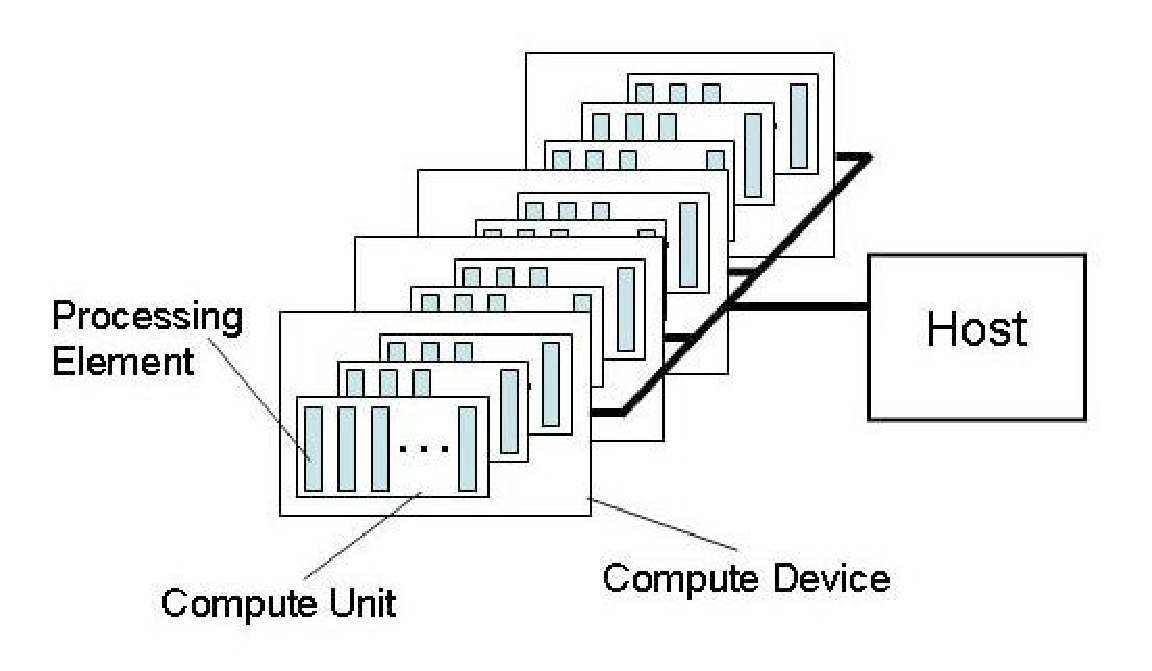
\includegraphics[width=8cm, height=4cm]{./eps/OpenCLArch.eps}
 \caption{OpenCL Architecture}
 \label{fig:OpenCLArch}
\end{figurehere}



\subsubsection{Application Execution, Work Items and Index Space}

From a very coarse point of view, we can describe the execution of an OpenCL application as a three-step process:

\begin{enumerate}
	\item when the application is launched, the \textbf{host} is executed on the CPU to define the \textbf{program context} (Section \ref{sect:context}) for the kernels and to dispatch them for execution.
	\item the \textbf{kernels} are executed on the OpenCL device(s) and compute their code over a stream of data.
	\item the resulting data is returned to the host.
\end{enumerate}

In OpenCL, an \emph{instance} of a kernel is called \textbf{work-item} and it executes over an \textbf{index-space} that contains the data. Multiple instances of a kernel can run simultaneously on the Coumpute Units of a Device (See \textbf{Figure \ref{fig:OpenCLArch}}).\\ Index spaces are basically the memory objects over which the work-items compute their istructions. In OpenCL index-spaces are also called \textbf{NDRange} (N-dimensional index space, where N can be a value of one, two or three, since GPUs can work on 1,2 or 3-dimensional textures).\\

\begin{figurehere}
 \centering
 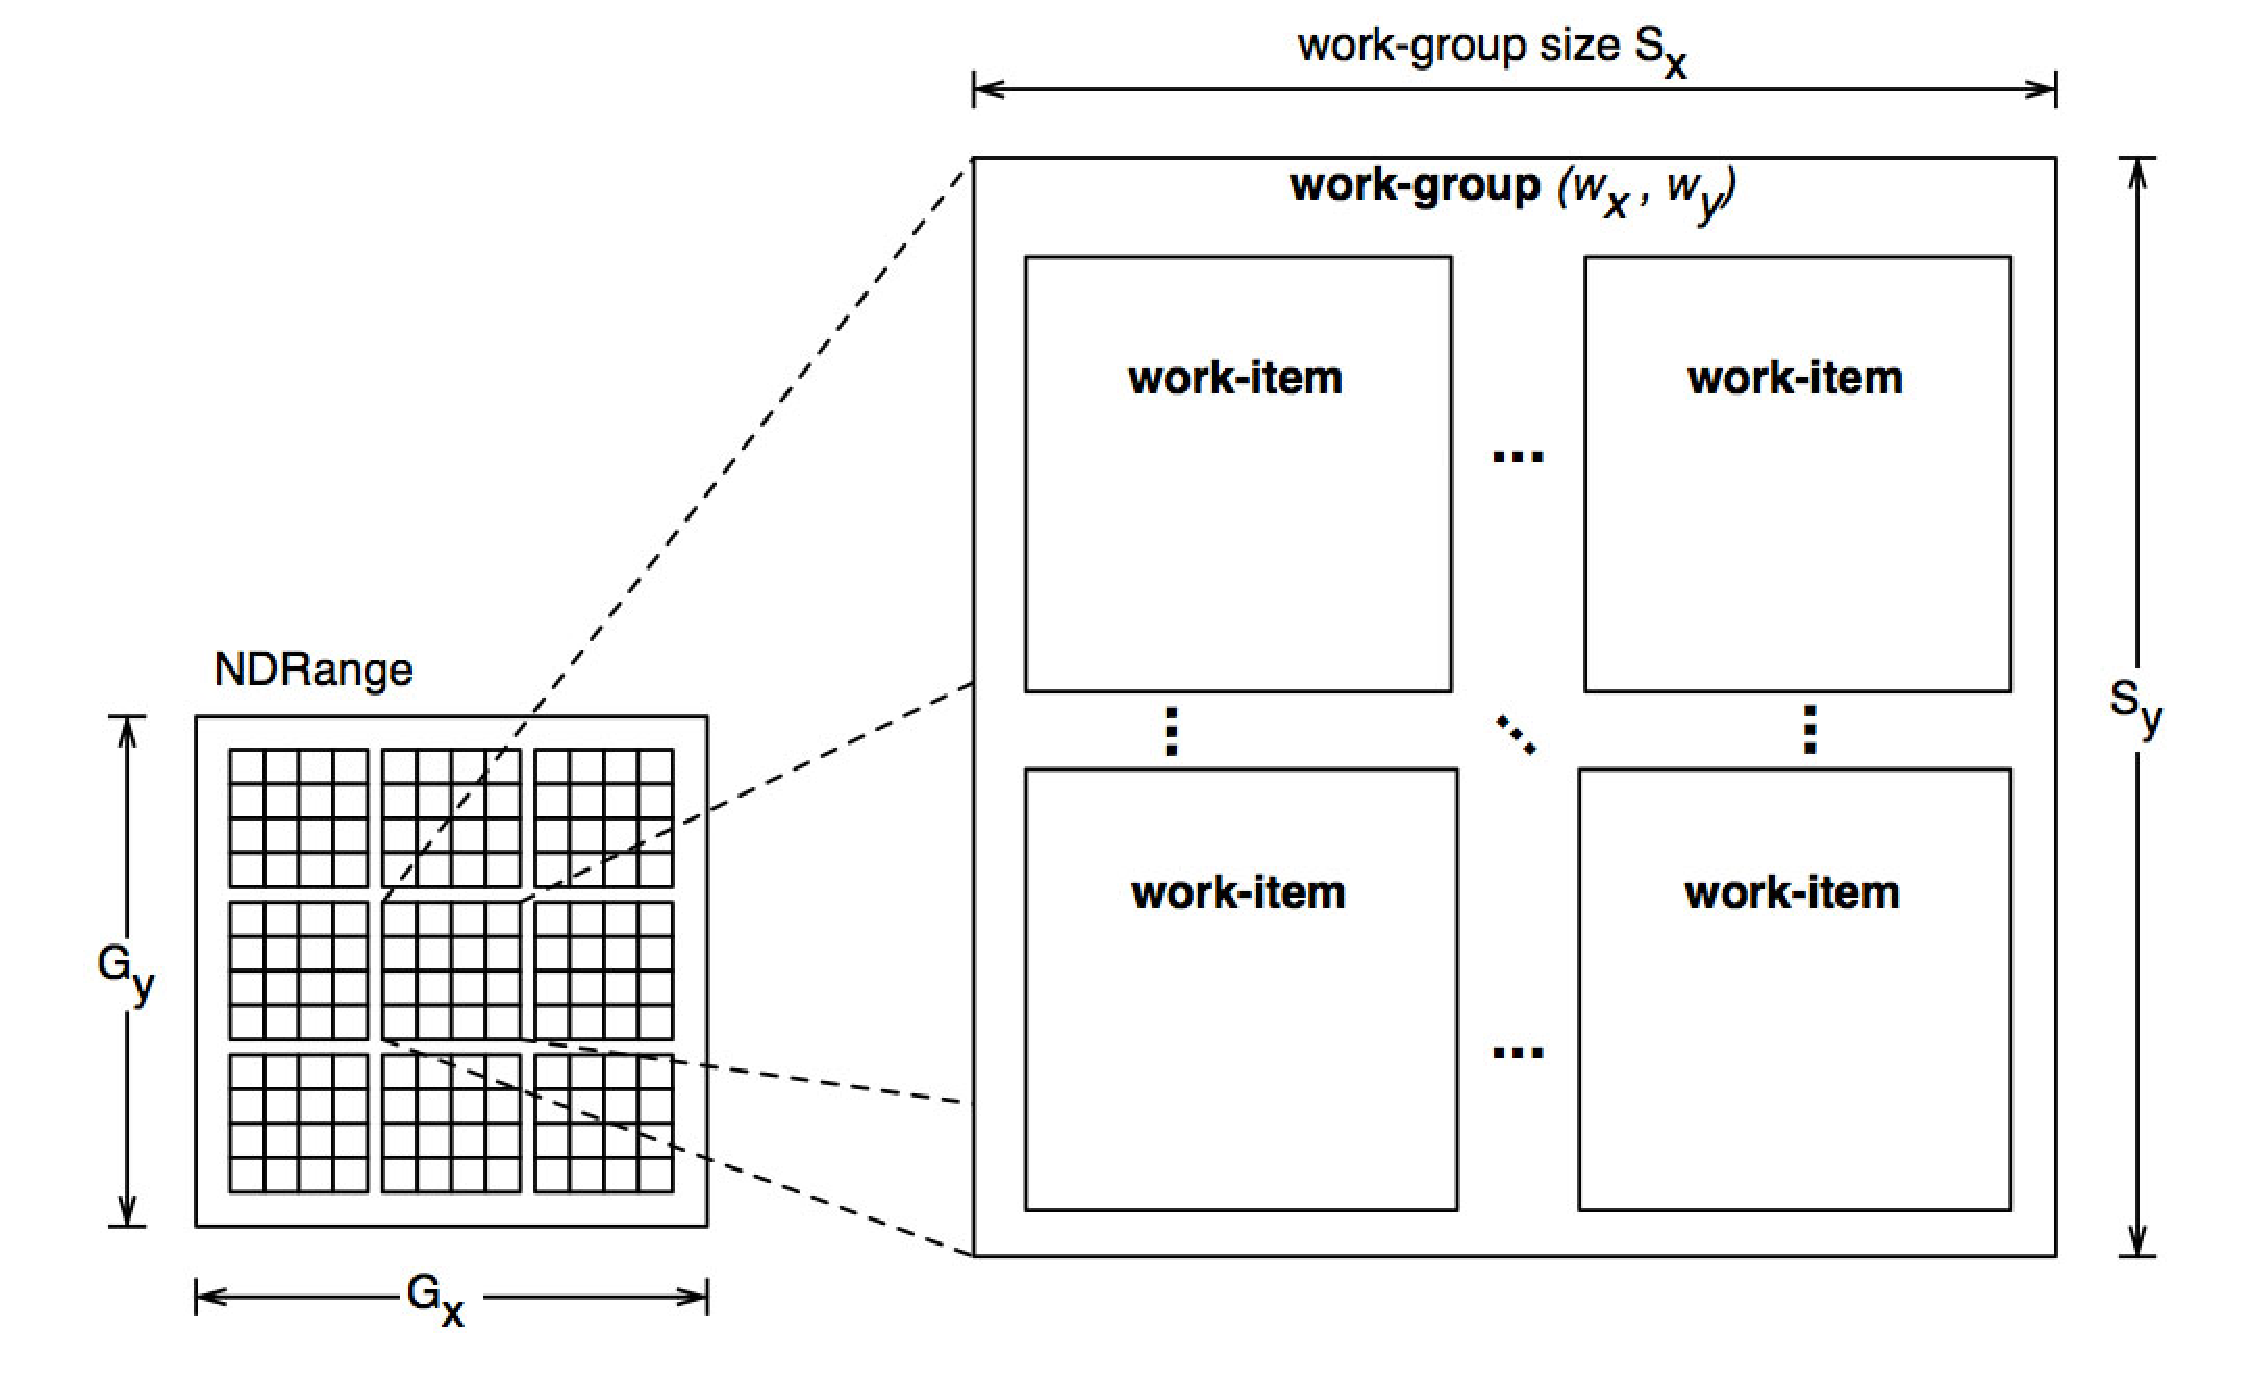
\includegraphics[width=8cm, height=4cm]{./eps/index-space.eps}
 \caption{Work-items mapped over a two-dimensional NDRange. As you can see, work-items can be organized in Work-Groups and every work-item has both a global and a local ID inside its work-group.}
 \label{fig:indexSpace}
\end{figurehere}

\begin{CLCode}
For example, to execute a kernel the host must call the \textbf{clEnqueueNDRangeKernel()} function. As you can see from the function name, kernels are not simply 'executed' but they must be enqueued in a specific command-queue, and they work over a NDRange memory object.
\end{CLCode}

\subsubsection{Kernel Implementation} \label{sect:kernelImplementation}
Below is an example of a simple kernel that calculates the square of the input NDRange:

{\footnotesize\begin{verbatim}
__kernel void myKernel(__global int* input,
                       __global int* output)
{
    int workID = get_global_id(0);
    output[workID] = input[workID] * input[workID];
}\end{verbatim}}

As you can see, a kernel is nothing different from a normal C/C++ function. The interesting thing of a kernel, is that it executes over \emph{each element} of the input memory object, even if no iteration is specified. This is due to the fact that when a kernel is dispatched for execution, it automatically creates multiple ``copies'' of the function (the work-item), each one with its own \textbf{workID} that maps directly to the NDRange. Each work-item has its own local environment that can be accessed using the work-item related function that the OpenCL API offers:\\

\begin{tablehere}
{\footnotesize
\begin{tabular}{|p{3,5cm}|p{3,5cm}|}\hline
\textbf{get\_work\_dim} & Number of dimensions in use\\ \hline
\textbf{get\_global\_size} & Number of global work items\\ \hline
\textbf{get\_global\_id} & Global work item ID value\\ \hline
\textbf{get\_local\_size} & Number of local work items\\ \hline
\textbf{get\_local\_id} & Local work item ID\\ \hline
\textbf{get\_num\_groups} & Number of work groups\\ \hline
\textbf{get\_group\_id} & Work group ID\\ \hline
\end{tabular}}
  \caption{Work-Item Built-In Functions\\}
	\label{tab:workItemFunctions}
\end{tablehere}


\subsubsection{Program Context and Command-Queue} \label{sect:context}

As we alreaty mentioned, one of the host functions is to define the \textbf{context} for the application. Contexts are used by the OpenCL runtime for managing objects such as command-queues, memory, program and kernel objects and for executing kernels on one or more devices specified in the context.\\
It basically consists in:

\begin{enumerate}
	\item a collection of \textbf{OpenCL devices} to be used
	\item a collection of the functions that will be executed on the devices (the kernels)
	\item \textbf{program objects}, that are simply the source files and executables that implements the kernels
	\item \textbf{memory objects}: the NDRange objects to be elaborated
\end{enumerate}

After the context has been created, the host initialize a structure called \textbf{command queue} that is used to schedule and dispatch commands to the devices within the context. The command structure is very simple and the commands that the host may issue fall only into three categories:

\begin{enumerate}
	\item \textbf{Kernel execution commands}: Execute a kernel Processing Elements of a device.
	\item \textbf{Memory commands}: Transfer data to, from, or between memory objects, or map and unmap
memory objects from the host address space.
	\item	\textbf{Synchronization commands}: Used to specify the order of execution of commands and to synchronize the kernels.
\end{enumerate}

\begin{CLCode}
Context and Command Queues are created by simply calling the \textbf{clCreateContext()} and \textbf{clCreateCommandQueue() 
} functions in the host.
\end{CLCode}


\subsubsection{The Memory}

There are four types of memory regions in OpenCL: \textbf{Global Memory}, \textbf{Constant Memory}, \textbf{Local Memory} and \textbf{Private Memory}.

\begin{itemize}
	\item Global memory grants read/write privileges to \textbf{all} the work-items in every work-group. Basically, every work-item (\emph{that are part of the same context}) can access it.
	\item Constant memory is only used to store constants. Only the host has write privileges over it, while kernels can only read from it.
	\item Local memory is shared among all the work-items that form a group. The host has no access to this memory area.
	\item Private memory is allocated directly by the work-item and can be used only by itself. The host has no access to this part of memory.
\end{itemize}

Since computation is carried on parallely, one of the major issues about memory is \textbf{consistency}. OpenCL uses a relaxed consistency memory model: the state of memory visible to a work-item is not guaranteed to be consistent across the collection of work-items at all times. \textbf{Table} \ref{tab:memconsistency} summarizes memory consistency for the various regions of memory available.\\

\begin{tablehere}
{\footnotesize
\begin{tabular}{|p{2cm}|p{5,5cm}|} \hline
\textbf{Memory} & \textbf{Consistency}\\ \hline
Private & memory is not shared, read/write consistency is always guaranteed\\ \hline
Local & consistency is guaranteed between work-items of the same work-group\\ \hline
Global & consistency is guaranteed between work-items of the same work-group, but not between multiple work-groups in the case they are assigned to execute the same kernel\\ \hline
\end{tabular}}
\caption{Memory consistency\\}
\label{tab:memconsistency}
\end{tablehere}
%\vfill
%\columnbreak
In OpenCL computation is performed over \textbf{memory objects}. There are two distinct memory objects: \textbf{buffers} and \textbf{images}.

\begin{itemize}
	\item Buffers are used to store a one-dimensional collection of elements (like an array), and those elements can be scalar values (int, float, etc.), vectors or user defined structures.
	Buffers are stored sequentially and \emph{can be accessed using pointers}; elements of a buffer are stored in memory in the \emph{same format} as they are used by kernels (i.e. if the kernel works on single integers, these elements are stored in memory as integers, this is not true for image objects)
	\item Images are used to store bi- or three-dimensional structures and their elements can only be selected from a list of predefined image formats (i.e. you cannot simply declare int or floats in an image object). Differently from buffers, elements of images \emph{cannot be accessed directly with a pointer} and they are \emph{always stored in memory as 4-dimensinal vectors} (since graphic shaders work on RGB and Alpha components of the pixels of an image)
\end{itemize}

\begin{CLCode}
In OpenCL memory objects are stored into \textbf{cl\_mem} structs, that can be easily initializated with the \textbf{clCreateBuffer()} and \textbf{clCreateImage()} functions.\\
Image format availables may vary from one graphic adapter to another, a list of supported image formats can be obtained using the \textbf{clGetSupportedImageFormats()} query.
\end{CLCode}



%-----------------------------------------------------------------------------
\vfill
\columnbreak
\subsection{Device Fission Introduction}

Device Fission is an extension of the OpenCL specification (fully defined in OpenCL 1.2, although is already available in OpenCL 1.1 as well as an optional extension) that adds a whole new level of control over parallel computation and hardware management.\\
As the term 'fission' implies (dividing or splitting something into two or more parts), device fission allows the sub-dividing of a device into one or more virtual sub-devices. This practice, when used carefully, can provide a huge performance boost, especially when executing parallel code on the CPU instead of the GPU \cite{intel:12:DeviceFission} (At present day device fission is suported only on CPUs and not on GPUs \cite{gaster:11:DeviceFission})
Implementing applications that use device fission \emph{does} require some knowledge of the underlying target hardware and, if not used properly, it can lead to worst performances and it may impact code portability.

\subsubsection{Device Fission as a better way to manage Embedded Systems}
Device fissioning can be very useful in embedded environments and, in general, in any situation where the system resources are limited:

\begin{itemize}
	\item Device fission allows to use only a \emph{portion} of a device, this means that the OpenCL runtime will not take the entire device for itself and other non-OpenCL application can work on it at the same time.\\ It can also help to reduce power consumption since high-task parallelism at low core frequencies can give better power perfomaces \cite{leskela:mobileGPGPU}
	\item Device fission allows to implement specialized memory sharing models that can be useful when it comes to manage the limited memory of an embedded system. (For example see the partitioning by affinity domain described in Section \ref{sect:memproximity})
	\item Since embedded systems may have limited graphic capabilities (or no graphic adapter at all), Device Fission may help to better exploit parallel computation where the only option is to use a CPU and not a GPU
\end{itemize}

\subsubsection{Sub Devices} \label{sect:DF-subdevices}
Each subdevice can have its own \textbf{program context} and \textbf{command-queue} (See Section \ref{sect:context}), this means that each subdevice can have its own private area of memory and that kernels can be dispatched independently to one subdevice or another.\\

\begin{CLCode}
In OpenCL you can create new sub-devices using the \textbf{clCreateSubDevices()} function. The first parameter to pass is of type \textbf{cl\_device\_id} and it is the ID of the 'parent' device to be partitioned. You can query for a list of available devices on the system by using the \textbf{clGetDeviceIDs()} function. Each sub-device can have a maximum number of compute units specified by the \textbf{CL\_DEVICE\_PARTITION\_MAX\_COMPUTE\_UNITS} property.
Since sub-devices are treated in the same exact way as 'normal' devices, different contexts and command-queue can be created by simply passing the ID of the subdevice to the \textbf{clCreateContext()} and \textbf{clCreateCommandQueue()} functions .
\label{Code:DevicePartitioning}
\end{CLCode}

There are three main way to partition a device: \textbf{equally}, \textbf{by counts} and \textbf{by affinity domain}:

\begin{itemize}
	\item partitioning a device \textbf{equally} means that the application will try to split the device into as many sub-devices as possible, each containting a number of Compute Units specified by the programmer. If that number does not divide evenly into the maximum available compute units, the remaining are not used.
	\item \textbf{by counts} means that the device is not divided automatically (and equally), but accordinlgy to a list provided by the programmer (e.g. given the list (4, 8, 16) the device will be divided into three sub-devices containing respectively 4, 8 and 16 CUs)
	\item partitioning by \textbf{affinity domain} is an automatic process that will create sub-devices composed of CUs that share similar levels of cache-hierarchy (specified by the programmer, e.g. L1, L2, L3 caches or NUMA nodes). This can be very useful when micro-management of memory is useful or for system where memory is a critical factor (for example in  embedded systems)
\end{itemize}

A list of some examples on how these partitioning parameters can be used to create different configurations on the same hardware can be found in the \textbf{Appendix A}.\\
Another interesting feature that allow even more flexibility and control over the hardware is that device fission allows sub-devices to be further partitioned and therefore create a tree-like structure like the one shown in \textbf{Figure \ref{fig:subdevicestree}}:

\begin{figurehere}
 \centering
 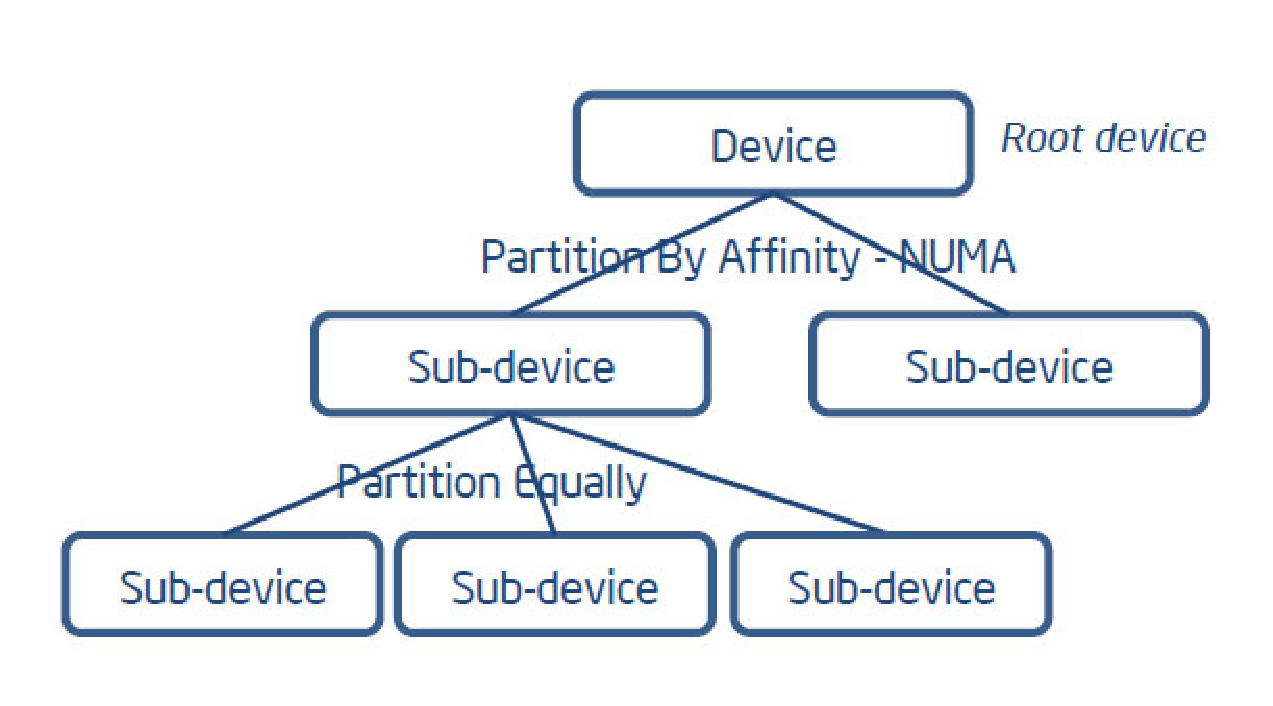
\includegraphics[width=8cm, height=4cm]{./eps/partitionTree.eps}
 \caption{Sub-devices can be further partitioned to create an hierarchy of devices. Each node of the tree can be partitioned using different partition parameters.}
 \label{fig:subdevicestree}
\end{figurehere}

\subsection{Device Fission Strategies}
Device fission can be used in several way to increase performance of OpenCL applications and to manage the (limited) resources of a system in a more efficient way. There are several standard approaches in which device fission can make the difference if used correctly.

\subsubsection{High-Priority dedicated sub-device} \label{sect:highPriority}
\begin{figurehere}
 \centering
 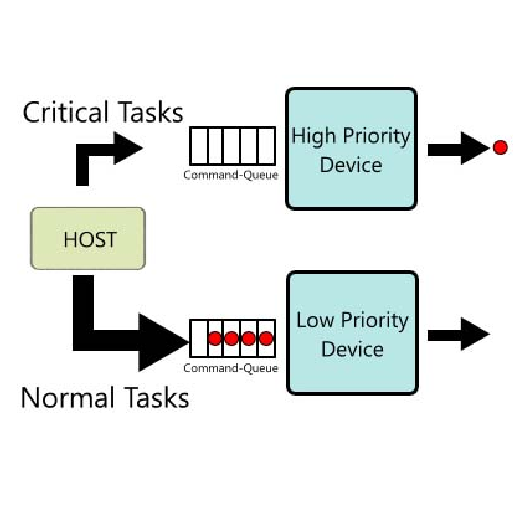
\includegraphics[width=6cm, height=6cm]{./eps/HighPriority.eps}
 \caption{Scenario 1: a sub device is created to compute high-priority tasks}
 \label{fig:highPriority}
\end{figurehere}

In this scenario, a sub-device is created to deal with critical tasks, while the remaining Compute Units of the device will be used for standard computation.
This configuration can be simply achieved by partitioning the device \textit{by counts}, reserving a few cores for high-priority computation and leaving the rest for normal computation.\\
The following code demostrates how to partition the device properly, the full code for this scenario can be found in \textbf{Appendix B}.


{\footnotesize\begin{verbatim}

// Get Device ID from platform [0]
// a list of available platforms can be obtained
// using clGetPlatformIDs() function

clGetDeviceIDs( platforms[0], CL_DEVICE_TYPE_CPU,
                1, &device_id, NULL);
								
// Create two sub-devices, the parameters for the
// partitioning are storend into a 
// cl_device_partition_property array

cl_device_partition_property param[5];
param[0] = CL_DEVICE_PARTITION_BY_COUNTS;
param[1] = 2;   // 1st device: 2 compute units
param[2] = 4; 	// 2nd device: 4 compute units
param[3] = CL_DEVICE_PARTITION_BY_COUNTS_LIST_END;
param[4] = 0; //end of list

//now we can create the sub-devices
cl_device_id output_IDs[2]; 
clCreateSubDevices(device_id, param, 2,
                   output_IDs, NULL);
									
//our `High Priority' device:
cl_device_id *hpDevice = &output_IDs[0];  
//our `normal' device:    
cl_device_id *normalDevice = &output_IDs[1]; 

\end{verbatim}}

\subsubsection*{Test Results}
In this scenario we created two sub-devices, one with 3 Compute Units (the low-priority one) and one with just one CU (the high-priority one) and tried to dispatch different sets of kernels marked 'normal' and 'critical'. First we dispatched all of them only to the low-priority device, and the result was that the tasks were completed in the same exact order they were dispatched, so the critical tasks had to wait for other tasks to finish. Then we routed the high priority tasks to the dedicated subdevice, with the result that those tasks were completed as soon as they were dispatched.\\
In another test we decided to stall the low-priority subdevice with an infinite while loop: the normal tasks were not able to continue their execution, but the the critical ones were executed normally as soon as they were dispatched thanks to the different routing.

\subsubsection{Memory Proximity} \label{sect:memproximity}

\begin{figurehere}
 \centering
 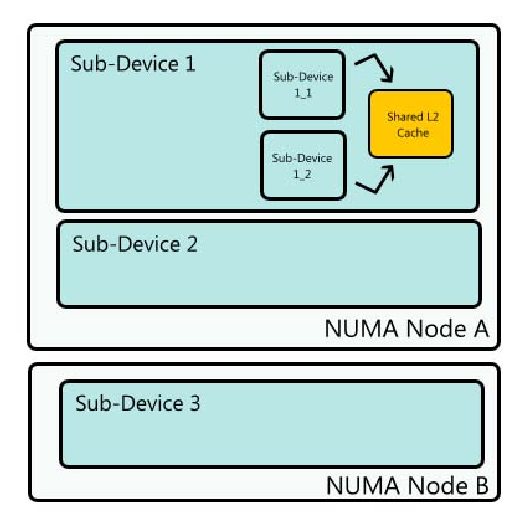
\includegraphics[width=6cm, height=6cm]{./eps/MemoryProximity.eps}
 \caption{The main device is partitioned into 2 subdevices that have Compute Units that share the same NUMA node. Subdevice 1 is further partitioned to obtain two devices that shares the same L2 Cache.}
 \label{fig:MemoryProximity}
\end{figurehere}

If the work-items of the application share high amounts of data, it can be useful to create sub-devices that share the same cache or are physically placed on the same NUMA node to icrease performance.
Without device fission, there is no guarantee that the work items will have these characteristics.
This kind of partitioning can be achieved using the \textit{partition by affinity model}, specifying which level of memory needs to be shared.
Obviously, this kind of partition is highly hardware-dependant, and it is not guaranteed that a particular partitionig scheme will work on different platforms.

\begin{CLCode}
The memory domains available on a particular device can be obtained by a simple query with the \textbf{clGetDeviceInfo()} passing \textbf{CL\_DEVICE\_PARTITION\_PROPERTIES} and \textbf{CL\_DEVICE\_PARTITION\_AFFINITY\_DOMAIN} as parameters.
\label{Code:MemoryDomains}
\end{CLCode}

The following example creates a partitioning model like the one shown in \textbf{Figure \ref{fig:MemoryProximity}}

{\footnotesize\begin{verbatim}
clGetDeviceIDs( platforms[0], CL_DEVICE_TYPE_CPU,
                1, &device_id, NULL);

// First partitioning
cl_device_partition_property params[3];
params[0] = CL_DEVICE_PARTITION_BT_AFFINITY_DOMAIN;
params[1] = CL_DEVICE_AFFINITY_DOMAIN_NUMA; 
params[2] = 0; // End of list

// Create the sub-devices:
cl_device_id subdevices_IDs[2];
clCreateSubDevices(device_id, params, 2,
                   subdevices_IDs, NULL);
									
// We devide the first subdevice into 2 further
// subdevices
cl_device_partition_property params[3];
params[0] = CL_DEVICE_PARTITION_BT_AFFINITY_DOMAIN;
params[1] = CL_DEVICE_AFFINITY_DOMAIN_L2_CACHE; 
params[2] = 0; // End of list

cl_device_id subsubdevices_IDs[2];
clCreateSubDevices(subdevices_IDs[0], params, 2,
                   subsubdevices_IDs, NULL);


\end{verbatim}}
\vfill
\columnbreak

\subsubsection{Warm Cores Exploitation}

\begin{figurehere}
 \centering
 \includegraphics[width=7cm, height=10cm]{./eps/WarmCores.eps}
 \caption{Without device fission there is no real control on which cores will be used, and tasks may be dispatched to 'cold' cores. With device fission we can redirect tasks to a specific (small) subdevice and exploit 'warm' cores.}
 \label{fig:WarmCores}
\end{figurehere}

Without device fission, when a new command is submitted to the command-queue it may happen that it will br dispatched for execution to a 'cold' core. 'Cold' cores are those that have cache memory filled with data that is not relevant to the current OpenCL program or task. With device fission we can force to use already 'warmed up' cores to minimize latency time.
This scenario adapts well for short-running programs, where the overhead of `warming' the core is relevant. For long-running programs, using device fission in this way may have very little effect or even degrade performance.
This approach can also be used for thermal management purposes, as it can have effect on which area of the CPU will heat more.\\
The implementation of this kind of behaviour is similar to the one described in Section \ref{sect:highPriority}: we can divide the device by \textit{counts}, reserving a 'warm' area over which we will dispatch fast and short tasks.

\subsubsection{Flowgraph and Pipeline Computation} \label{sect:pipelineScenario}

\begin{figurehere}
 \centering
 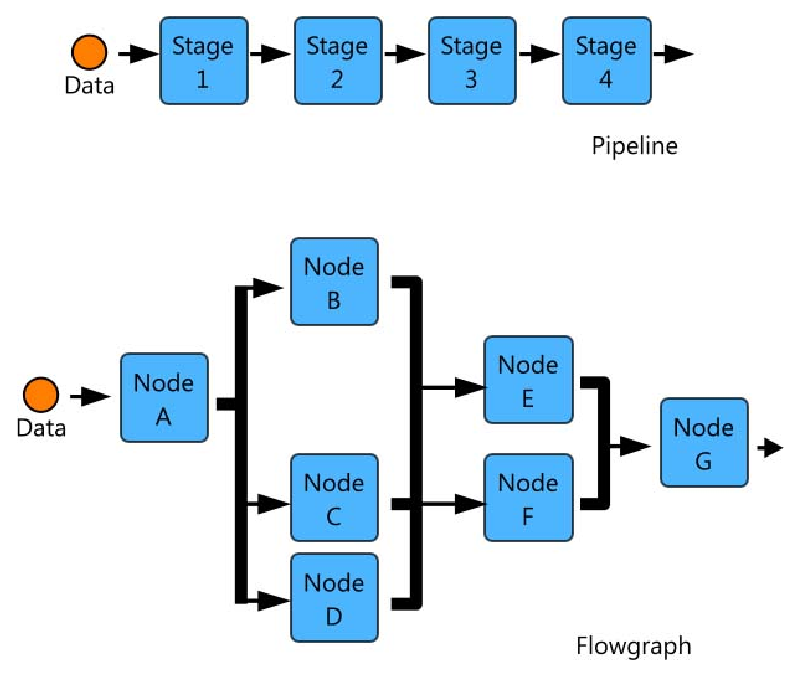
\includegraphics[width=8cm, height=7cm]{./eps/flow.eps}
 \caption{Device partitioning allows to create 'virtual' pipelines}
 \label{fig:flow}
\end{figurehere}

Since device fission gives total control over task dispatching, we can use it to create complex structures like 


\subsubsection{Maximize Throughput}
This scenario applies when data sharing is very limited or completely absent, and the only important thing is to maintain high levels of throughput. To achieve this, a job must have \textit{all the resources} available for itself (i.e. all the on-chip caches), and no other jobs may interfere, therefore we must create \emph{one and only one} device for each NUMA node, so no device can "`overlap"' resources with another.

SISTEMARE.......Use Partition By Affinity to create N sub-devices one sub-device for each NUMA node.
The sub-devices can then use all NUMA node's resources including all of the available cache.







\hyphenation{FPGA}
\hyphenation{FPGAs}

%%%%%%%%%%%%%%%%%%%%%%%%%%%%%%%%%%%%%%%%%%%%%%%%%%%%%%%%%%%%%%%%%%%%%%%%%%%%%
\section{Real World Examples and Case Studies of OpencCL and Device Fission Applications}


%------------------------------------------------------------------------------
\subsection{OpenCL for FPGA implementation}
The great flexibility of OpenCL allows it to run on a great variety of different hardware and platforms. One interesting application, expecially in the field of embedded systems, is to use it as substitute of traditional HDLs (Hardware Description Languages) like VHDL or Verilog when FPGA programming is required.

\subsubsection{OpenCL-FPGA Implementation}
As we already saw, OpenCL applications consists of two part: the host and the kernels.
When migrating to FPGA, the developer has to opt for two solutions:

\begin{enumerate}
	\item An ``All in One solution'', by implementing the CPU that will run the standard C/C++ host code directly on the FPGA. (For example by using a soft macro provided by the microprocessor manufacturer)
	\item A separated solution, by using an external microprocessor for the host and by programming the FPGA to execute the kernels only.
	\end{enumerate}
	
Unlike CPUs and GPUs, where parallel threads are executed on the different (and generic) cores available, FPGAs offer a different strategy. Kernel functions can be transformed into dedicated, specialized, and deeply pipelined \textbf{hardware circuits} that are inherently multithreaded thanks to the concept of pipeline parallelism. Each pipeline can then be replicated over the entire FPGA to provide even more parallelism. This two levels of parallelism translates into an immediate boost in performance.\\
\textbf{Figure \ref {fig:fpga_example}} shows a simple example of how kernels are translated into separate, multiple \textbf{hardware pipelines}.
	
\begin{figurehere}
 \centering
 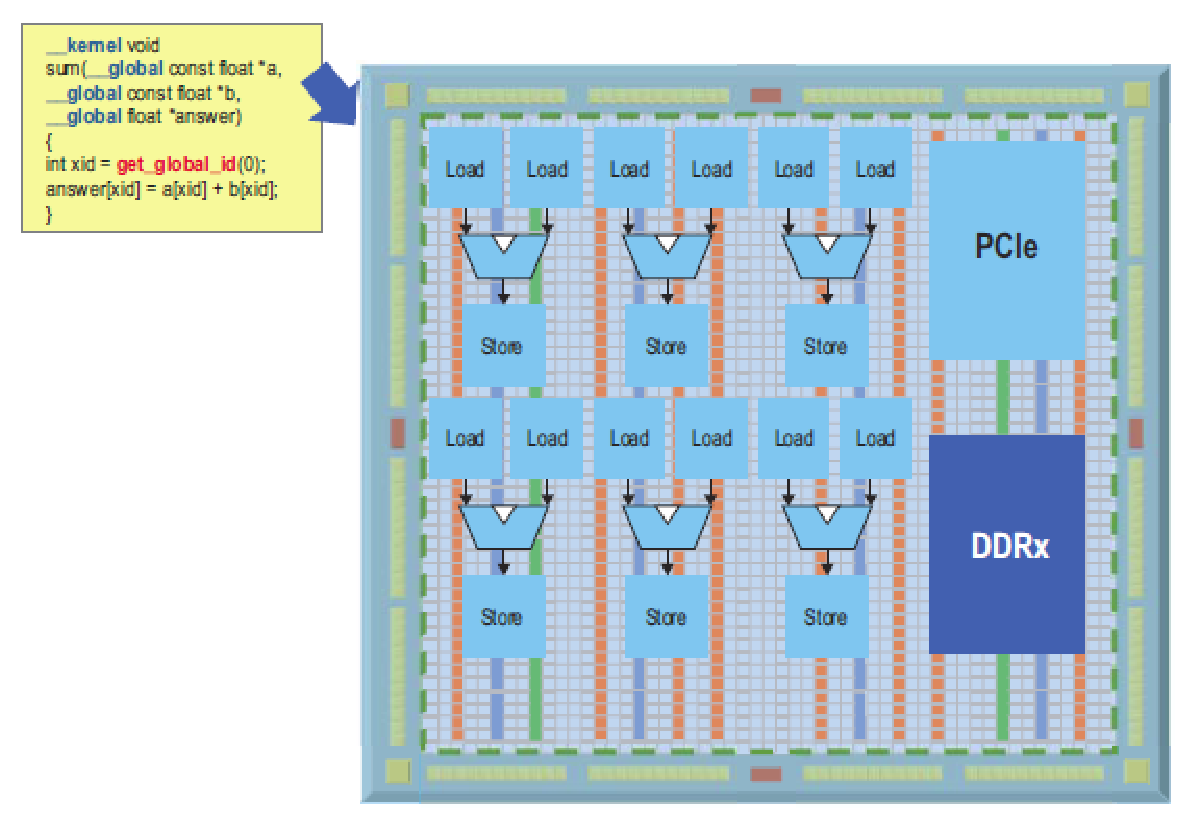
\includegraphics[width=8cm, height=4cm]{./eps/FPGA1.eps}
 \caption{Kernels are translated into multiple hardware pipelines, inherently providing two levels of parallelism: pipeline parallelism and thread level parallelism}
 \label{fig:fpga_example}
\end{figurehere}

The most important concept behind the OpenCL-to-FPGA approach is the notion of \textbf{pipeline parallelism}.
Basically, an OpenCL-to-FPGA compiler is able to implement the scenario observed in Section \ref{sect:pipelineScenario} in an automatic and more efficient way. We will describe how pipeline parallelism work by introducing an example, shown in \textbf{Figure \ref{fig:fpga_example2}}:

\begin{figurehere}
 \centering
 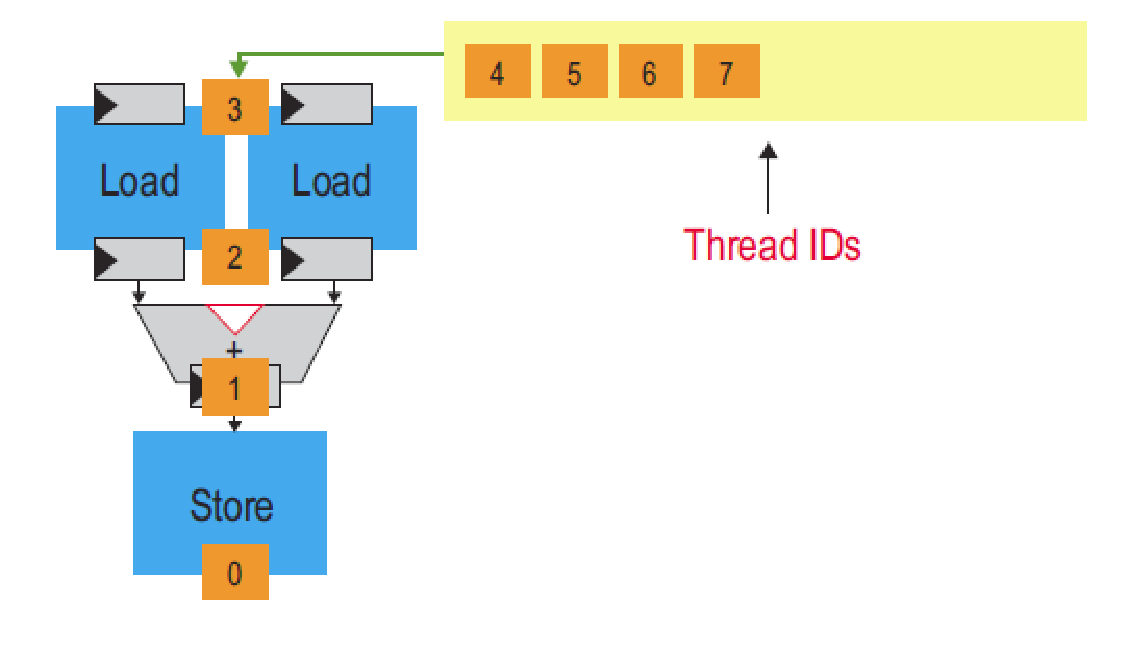
\includegraphics[width=8cm, height=4cm]{./eps/FPGA2.eps}
 \caption{Pipeline parallelism example}
 \label{fig:fpga_example2}
\end{figurehere}

On the first clock cycle, thread 0 is clocked into the two load units. This indicates that they should begin fetching the first elements of data from arrays A and B. On the second clock cycle, thread 1 is clocked in
at the same time that thread 0 has completed its read from memory and stored the results in the registers following the load units. On cycle 3, thread 2 is clocked in, thread 1 captures its returned data, and thread 0 stores the sum of the two values that it loaded. It is evident that in the steady state, all parts of the pipeline are active, with each stage processing a different thread.
	
In \textbf{Figure \ref{fig:fpga_implementation}} you can see a general scheme that summarizes how OpenCL-FPGA applications should be implemented. Since memory is shared between all the components, one crucial point in parallel computation is the memory management, and as we can see from the figure several memory interfaces are needed, but generally OpenCL-FPGA compilers are able to implement such interfaces automatically, exempting the developer from such tedious and delicate task.

\begin{figurehere}
 \centering
 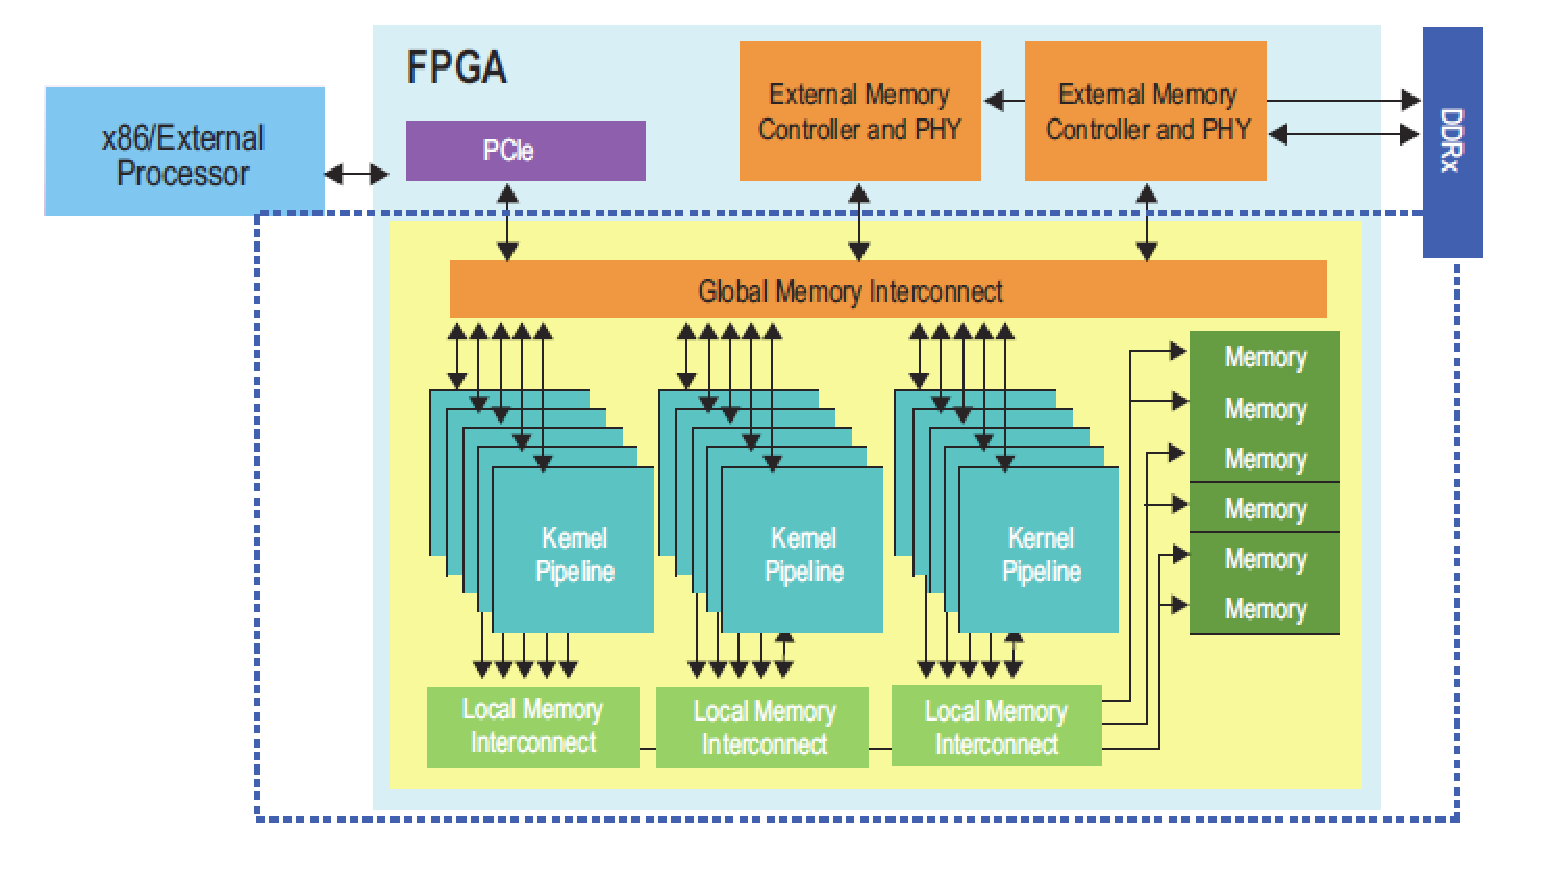
\includegraphics[width=8cm, height=4cm]{./eps/FPGA3.eps}
 \caption{OpenCL-FPGA Implementation scheme}
 \label{fig:fpga_implementation}
\end{figurehere}

\subsubsection{Benefits}

Using OpenCL as a substitute of traditional HDLs can provide various benefits:

\begin{itemize}
	\item \textbf{Improved Time To Market:} OpenCL offers a quicker and simpler way to implement parallel alghorithms  compared to traditional FPGA development using lower level hardware description language (HDLs) such as Verilog or VHDL \cite {altera:FPGA}.  This because OpenCL inherently offers the ability to describe parallel computation, while the main challenge in HDLs languages was exactly to extract thread-level parallelism from a sequential program. OpenCL offers instead the ability to the programmer to specify and control parallelism in an explicit and clear way.
	\item \textbf{Better Performance:} Dedicated ad-hoc hardware structures allow faster computation than using generic CPUs. Furthermore OpenCL-FPGA compilers automatically exploit pipeline parallelism to make computation even faster.
	\item \textbf{Less Power Consumption:} Benchmarks show that FPGA applications consumes lot less power to execute the same OpenCL code in comparison to CPU or GPU solutions.
\end{itemize}

\subsubsection{Case Study: Monte Carlo Black-Scholes Method}

In this experiment an economic model was used to benchmark an OpenCL-FPGA unit. The model is based on the 
Monte Carlo Black-Scholes method and it is used to compute the expected payoff of stock prices over millions of different paths. The entire algorithm used for this benchmark can be implemented in approximately 300 lines of
OpenCL code that is portable from FPGA to CPU and GPU. The comparison in performance  between these 3 different platforms are shown in \textbf{Table \ref{tab:FPGABenchmark}}.\\

\begin{tablehere}
{\footnotesize
\begin{tabular}{|p{1,0cm}|p{1,8cm}|p{1,8cm}|p{1,8cm}|}\hline
\textbf{Platform} & \textbf{Power} [Watts] & \textbf{Performance} [Billions of simulations per seconds] & \textbf{Efficiency} [Millions of simulations per second per watt]\\ \hline
CPU & 130 & 0.032 & 0.0025 \\ \hline
GPU & 212 & 10.1 & 48 \\ \hline
FPGA & 45 & 12.0 & 266 \\ \hline
\end{tabular}}
  \caption{Monte Carlo Black-Scholes benchmark results\\}
	\label{tab:FPGABenchmark}
\end{tablehere}

As we can see, not only the OpenCL framework targeting a FPGA board exceeds the throughput of both a CPU and a GPU, but it also consumes one-fifth the power of comparable GPUs when executing the same code.

\subsubsection{Case Study: Document Filtering}

In this benchmark the focus is set on a more practical problem than the previous, as it will consider an algorithm used in modern data centers.
A recent report \cite{walsh:power} from International Data Corporation (IDC) examined the requirements of high performance computing data centers, and conducted a survey of the top constraints in expanding current data center capabilities. From the results, it was obvious that power and cooling costs are the key impediments of compute capability expansion, and as we have seen in the previous benchmark, FPGA computation offer an huge improvement in power consumption.\\
In this experiment, a document filtering algorithm was implemented using OpenCL to program an FPGA. The algorithm basically consists in analyzing an incoming stream of documents and find the ones that best match a user's interest. The results are shown in \textbf{Table \ref{tab:FPGABenchmark2}}:\\

\begin{tablehere}
{\footnotesize
\begin{tabular}{|p{1,0cm}|p{1,8cm}|p{1,8cm}|p{1,8cm}|}\hline
\textbf{Platform} & \textbf{Power} [Watts] & \textbf{Performance} [Million of Terms per seconds] & \textbf{Efficiency} [Millions of Terms per Joule]\\ \hline
CPU & 130** & 2070 & 15.9 \\ \hline
GPU & 215 & 3240 & 15.1 \\ \hline
FPGA & 21 & 1755 & 83.6 \\ \hline
\end{tabular}}
  \caption{Document Filtering benchmark results\\ **Does not include memory consumption.\\}
	\label{tab:FPGABenchmark2}
\end{tablehere}

As you can see, although CPUs and GPUs can perform better in terms on throughput, the power efficiency of these two platform can be five time lower than the efficiency of FPGAs. It is interesting to note that in this case the performance of the FPGA was limited by the external memory bandwidth, and not by the FPGA itself. With a proper setup, the authors of this test extimate an increase in performance up to 2925 MT/s maintaining the same power consumption level, that would raise the power efficiency value from 83.6 MT/J to 139,3 MT/J.\\
These results demonstrate that introducing an FPGA OpenCL implementation of algorithms, could bring a dramatic decrease of power consumption and thus cooling costs in modern data centers.


%-----------------------------------------------------------------------------

\subsection{Investigating performance portability of OpenCL}

In the next example \cite{Pennycook2012} OpenCL was used to re-implement an existing benchmark algorithm to see how well it performs against the native implementation of the code. The results are very interesting and surprising, and they pave the way for a complete new point of reflection.\\
The second part of the experiment shows instead how the introduction of Device Fission to better use the memory allow to obtain considerable speedups over the unmanaged version of the same code.

\subsubsection{Background: the LU algorithm}

LU is an application level benchmark part of the NPB Suite (NAS Parallel Benchmark) that consists in a series of parallel aerodynamic simulations designed by NASA. LU is short for Lower-Upper Gauss-Seidel solver and the algorithm is basically a simplified Navier-Stokes equation solver that uses three-dimensional data grid for its calculations. The size of these data cubes is always \begin{math}N^3\end{math}, and for the purpose of this example we'll focus only on three specific classes of problems: Class A problems (size \begin{math}64^3\end{math}), Class B problems (size \begin{math}102^3\end{math}) and Class C problems (size \begin{math}162^3\end{math}).
To perform the calculations, each cube of size \begin{math}n\times n\times n\end{math} is divided into 2D ``slices'' of size \begin{math}n\times n\times 1\end{math}, and each ``slice'' is assigned to a different processor for computation. This algorithm is further optimized used a technique called \textit{k-blocking}; \textbf{Figure \ref{fig:dataCubes}} shows a visual representation of how data is explored, as you can see each block must wait for the adjacent block to be completely computed (the black ones) before computation can start.\\

\begin{figurehere}
 \centering
 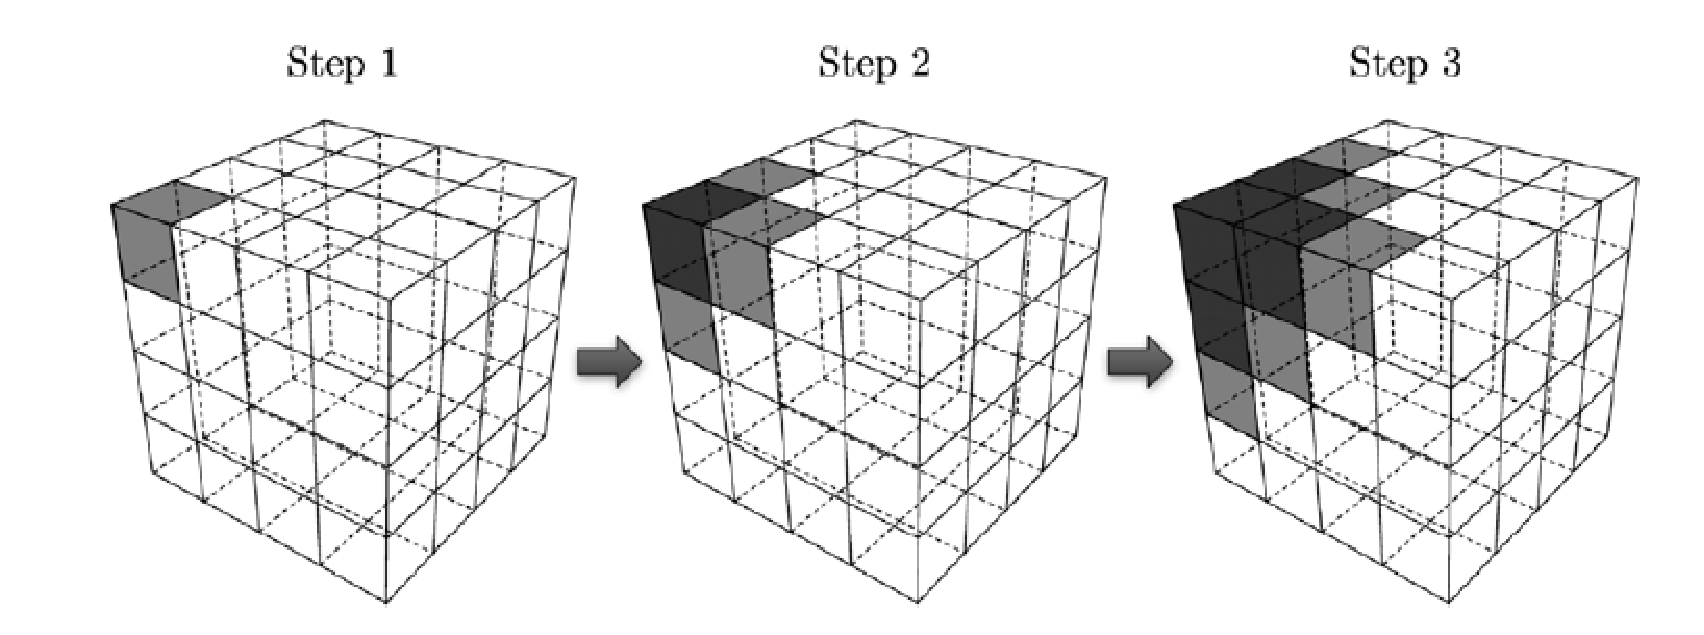
\includegraphics[width=8cm]{./eps/dataCube.eps}
 \caption{Data cubes used in the LU algorithm}
 \label{fig:dataCubes}
\end{figurehere}


\subsubsection{The Experiment}

\textbf{Table \ref{tab:LUBenchmark1}} shows a list of the devices used in the experiment. One important aspect of OpenCL to note is its \textbf{code portability}: the same source code can be used on different devices with different numbers of cores and processing units, as OpenCL is able to scale over them automatically. This property of OpenCl is not to be underevaluated and it already offers many benefits:\\

\begin{itemize}
	\item it is easier to maintain a single code that targets all platforms, as opposed to separate hand-tuned versions of the same code for each alternative platform.
	\item it reduces the risk of being locked into a single vendor solution.
	\item benchmarking is simplified, as the results can be compared from a single code source.
	\item it represents a ``safer'' investment for computing sites, as new codes (and ported legacy codes) will run on both existing and future architectures.
\end{itemize}

\begin{tablehere}
{\footnotesize
\begin{tabular}{|p{2,2cm}|p{2,0cm}|p{2,0cm}|}\hline
\textbf{Platform} & \textbf{Compute Units} & \textbf{Processing Elements} \\ \hline
Intel X5550, 2.66 GHz (x86 CPU) & 4 & 4 \\ \hline
Intel X5660, 2.80 GHz (x86 CPU) & 12 & 12 \\ \hline
NVIDIA Tesla C1060 (GPU) & 30 & 240 \\ \hline
NVIDIA Tesla C2050 (GPU) & 14 & 448 \\ \hline
AMD/ATI FirePro V7800 (GPU) & 18 & 1440 \\ \hline
\end{tabular}}
  \caption{Platforms used in the experiment.\\}
	\label{tab:LUBenchmark1}
\end{tablehere}

The goal of the first tests was to analyze the performances of OpenCL implementation of LU against native FORTRAN77 (for CPUs) and CUDA (for GPUs) implementations.\\ \textbf{Figure \ref{fig:OpenCLvsFORTRAN77}} shows the results of the comparison between OpenCL and FORTRAN77. Each implementation was compiled using two different compilers for each approach.

\begin{figurehere}
 \centering
 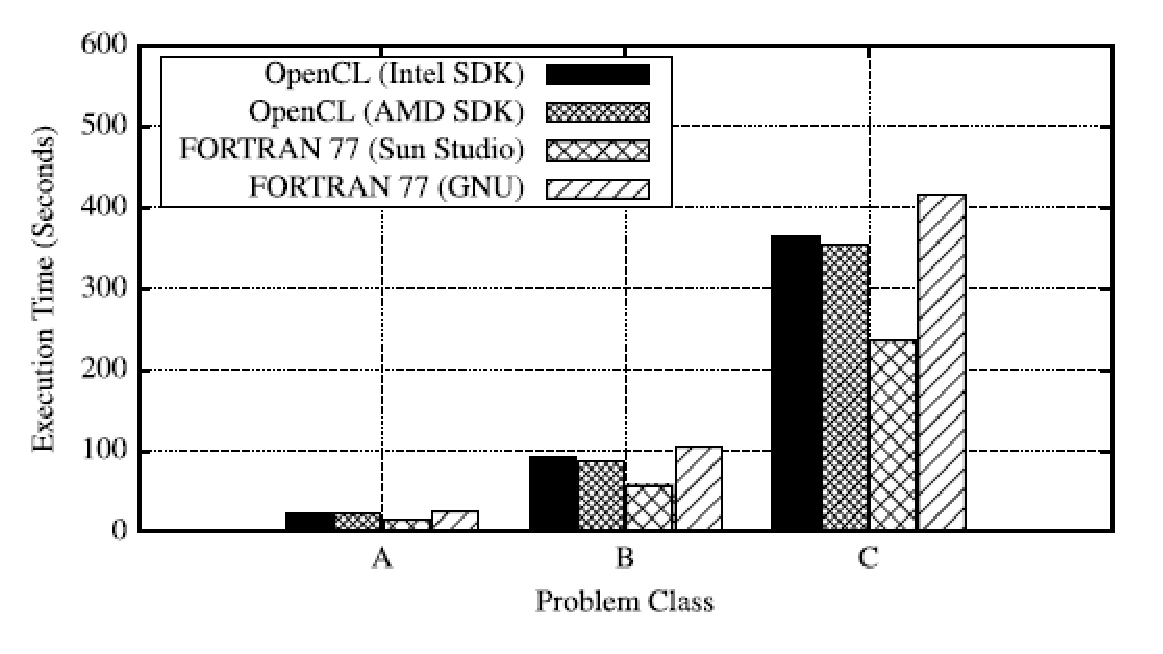
\includegraphics[width=8cm, height=4cm]{./eps/OpenCLvsFORTRAN77.eps}
 \caption{OpenCL vs Fortran Comparison}
 \label{fig:OpenCLvsFORTRAN77}
\end{figurehere}

As we can see from the graph the advantage of OpenCL (if any) is very marginal, and in the case of the Sun Studio compiler, the FORTRAN77 implementation performs way better. This result is very interesting because it demonstrates two things:

\begin{enumerate}
	\item that \emph{OpenCL is not always the best option in term of performance}
	\item that the compiler used can play a very important role
\end{enumerate}

The reason of this OpenCL ``failure'' could be indeed attributed to the fact that the FORTRAN compiler is very mature and has a long story of optimizations and fine-tuning behind it, while OpenCL standard is quite young; and another interesting thing that can be seen from the graph is that there is practically no difference in performance between the two versions of the OpenCL implementation, and this means that no compiler is better optimized that the other.\\
Let's now see how OpenCL perform against the CUDA implementation (GPU), the results are shown in \textbf{Figure \ref{fig:OpenCLvsCUDA}}:\\

\begin{figurehere}
 \centering
 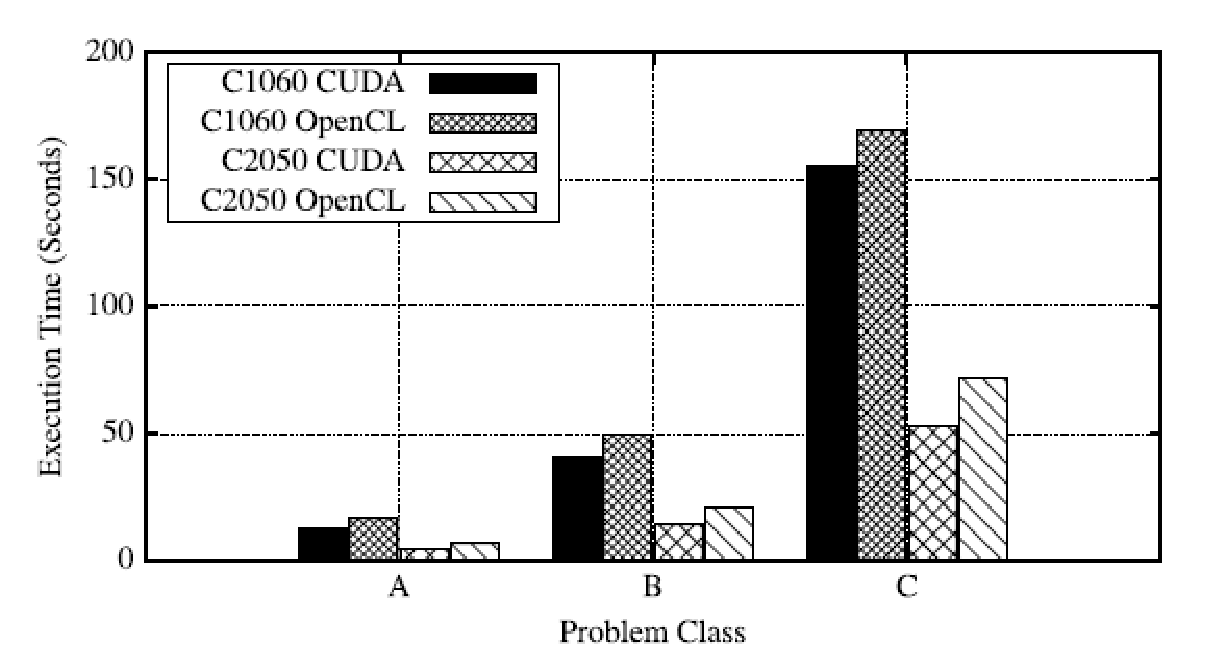
\includegraphics[width=8cm, height=4cm]{./eps/OpenCLvsCUDA.eps}
 \caption{OpenCL vs CUDA Comparison}
 \label{fig:OpenCLvsCUDA}
\end{figurehere}

As we can see even in this case the CUDA implementation performs a little better, and the reason in still to be searched into specific optimizations offered by the CUDA compiler for NVIDIA boards.

\subsubsection{Introducing Device Fission} \label{sect:LUDeviceFission}

The same benchmark will now be ran using device fissioning to exploit either temporal or spatial cache locality and therefore use the shared memory in a more efficient way. Previous executions of the benchmark were \emph{unlikely to exhibit good memory behaviour}, because basic OpenCL implementation has no control over which processing unit the work items will be allocated.\\
In the new test setup, the LU benchmark will be executed over 2 different configurations created with device fissioning (\textbf{Figure \ref{fig:LU_deviceFissionConfig}}): two subdevices with 6 compute units each and 4 devices with 3 compute units each.

\begin{figurehere}
 \centering
 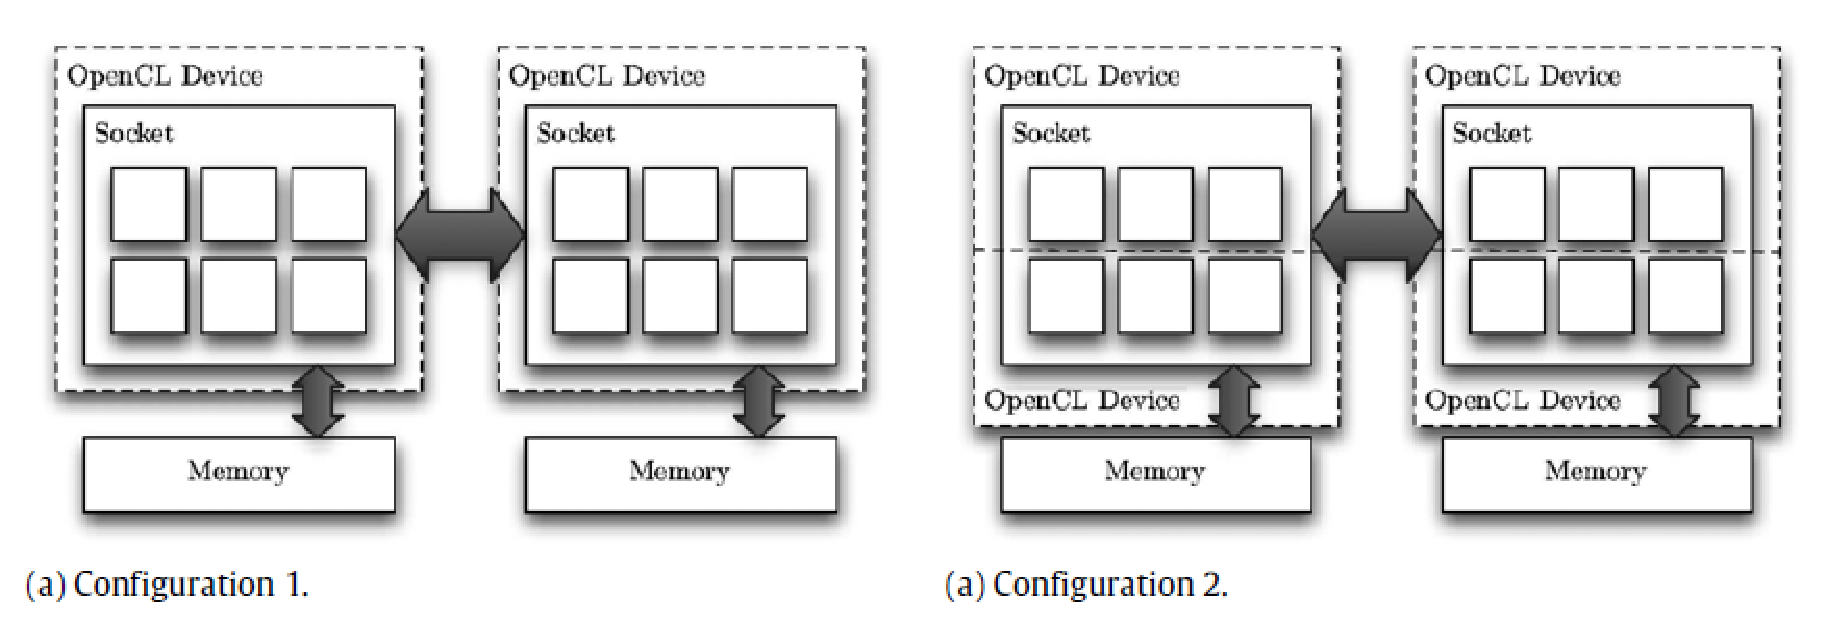
\includegraphics[width=8cm]{./eps/LU_deviceFissionConfig.eps}
 \caption{The two configurations used in the device fission tests}
 \label{fig:LU_deviceFissionConfig}
\end{figurehere}

The results of the test are listed in \textbf{Table \ref{tab:LUDeviceFission}}, and they clearly suggest that device fission can provide significant performance improvements when used and configured properly, with an average speedup of 2.56x. \\

\begin{tablehere}
{\footnotesize
\begin{tabular}{|p{1,7cm}|p{1,7cm}|p{1,7cm}|p{1,7cm}|}
\hline
       Num of Cores		& \multicolumn{1}{|p{1,55cm}}{With Device Fission}& \multicolumn{1}{|p{1,55cm}}{Witout Device Fission}& \multicolumn{1}{|p{1,55cm}|}{Speedup} \\ \hline
\multicolumn{1}{|l}{\textbf{Configuration 1}} & \multicolumn{1}{c}{}  & \multicolumn{1}{c}{}  & \multicolumn{1}{c|}{}  \\ \hline
      24  & \multicolumn{1}{|c}{568.56} & \multicolumn{1}{|c}{1158.60} & \multicolumn{1}{|c|}{2.03x} \\ \hline
			48  & \multicolumn{1}{|c}{397.41} & \multicolumn{1}{|c}{760.73} & \multicolumn{1}{|c|}{1.92x} \\ \hline
      96  & \multicolumn{1}{|c}{276.68} & \multicolumn{1}{|c}{503.25} & \multicolumn{1}{|c|}{1.81x} \\ \hline
      384  & \multicolumn{1}{|c}{123.75} & \multicolumn{1}{|c}{n.a.} & \multicolumn{1}{|c|}{n.a.} \\ \hline

\multicolumn{1}{|l}{\textbf{Configuration 2}} & \multicolumn{1}{l}{}  & \multicolumn{1}{l}{}  & \multicolumn{1}{l|}{}  \\ \hline
      12  & \multicolumn{1}{|c}{622.27} & \multicolumn{1}{|c}{1884.87} & \multicolumn{1}{|c|}{3.02x} \\ \hline
			24  & \multicolumn{1}{|c}{394.63} & \multicolumn{1}{|c}{1158.60} & \multicolumn{1}{|c|}{2.93x} \\ \hline
      48  & \multicolumn{1}{|c}{250.84} & \multicolumn{1}{|c}{760.73} & \multicolumn{1}{|c|}{3.03x} \\ \hline
      192  & \multicolumn{1}{|c}{100.71} & \multicolumn{1}{|c}{320.53} & \multicolumn{1}{|c|}{3.18x} \\ \hline
\end{tabular}}
  \caption{Runtimes (in seconds) for two device fission configurations.}
	\label{tab:LUDeviceFission}
\end{tablehere}

\subsubsection{Conclusions}
Even if at a first glance the results of this experiments may seem disappointing (OpenCL failed against FORTRAN and CUDA),
it brought to light one interesting point about OpenCL implementations: compiler optimization.
The main problem when using OpenCL is that calls to its functions are made by way of a library, and therefore the operation of these functions may not be necessarily defined until runtime, and this restricts the optimisation freedom of the host compiler. One solution to this problem may be a compiler that analyzes both the host \emph{and} the OpenCL code at the same time, producing an optimized but \emph{platform specific} code. Thus there is a conflict between potential compiler optimization and the vast code portability already provided by OpenCL: optimizing the compiler would make the code less portable.\\
The second part of the experiment shown instead a practical example on the strenght of device fission, as it could indeed offer the possibility to better manage the resources available and produce more performant code.


%---------------------------------------------------------------------------------------------------

\subsection{OpenCL remote clustering}
In this section we'll present an interesting example \cite{mosix:virtualcl} on how OpenCL can be used in a \emph{distributed} and \emph{heterogeneous} computer environment that can provide an opportunity to increase the performance of parallel and High-Performance Computing applications on clusters, by combining traditional multi-core CPUs, general-purpose GPUs and Accelerator devices.\\
One limitation of parallel computing using OpenCL is that most applications run their device-specific code (the kernels) only locally on the same computer were the hosts application runs.\\
Previous studies in this sector have already been made, and it has been demonstrated \cite{barak:heterogeneous} that OpenMP (one of the main paradigms for HPC parallel programming) can be extended to use a heterogeneous cluster environment by letting the CPU portion of the application run on one local node, and the GPU kernels on cluster-wide remote devices. In this example we will present a first attempt to extend OpenCL in a similar way.

\subsubsection{The VirtualCL Cluster Platform}
VirtualCL (VCL) is an OpenCL wrapper that allows most applications to transparently utilize remote OpenCL devices as if they all resided on the same local computer.\\
The basic idea behind this platform is to provide to the application the impression of having of a single host with many local devices, no matter where they phisically are. Users can launch the OpenCL executable on the host computer, then VCL manages and transparently runs the kernels on the different nodes available.
VCL is composed of three main components: the VCL library, the broker and the back-end daemon.\\
The \textbf{VCL library} is a cluster-wide front-end for OpenCL that gives applications transparent access to openCL devices in the cluster, hiding their actual location from the calling executable.\\
The \textbf{broker} is a daemon-process connected with the library via a UNIX socket that runs on every host computer. Its main tasks are to monitor for existence and availability of OpenCL devices in the cluster, to allocate them, and to authenticate and route messages between the applications and the back-ends.\\
The \textbf{back-end daemon} runs on each cluster node (and not the on the host, like the broker) and its goal is to execute kernels on behalf of the client application.

\subsubsection{VCL Performances}
One of the main factors that have to be taken into account when using a wrapper model like VCL is the \textbf{overhead} introduced by it. To evaluate it it is sufficient to measure the time taken by the application to run a sequence of identical kernels using the native OpenCL library locally and then the time to run the same kernels with VCL both on local and remote devices. The results for overhead testing are shown in \textbf{Table \ref{tab:VCLOverhead}} and it is clear that the difference between local and remote use of VCL is very small (about 80 milliseconds) and almost independent from the size of the buffer used.\\

\begin{tablehere}
{\footnotesize
\begin{tabular}{|p{1,65cm}|p{1,65cm}|p{1,65cm}|p{1,65cm}|}\hline
\textbf{Buffer Size} & \textbf{Native OpenCL Time} [ms] & \textbf{VCL Overhead (Local)} [ms] & \textbf{VCL Overhead (Remote)} [ms]\\ \hline
4 KB & 96 & 35 & 113 \\ \hline
16 KB & 100 & 35 & 111 \\ \hline
64 KB & 105 & 35 & 106 \\ \hline
256 KB & 113 & 36 & 105 \\ \hline
1 MB & 111 & 34 & 114 \\ \hline
4 MB & 171 & 36 & 114 \\ \hline
16 MB & 400 & 36 & 113 \\ \hline
64 MB & 1354 & 33 & 112 \\ \hline
256 MB & 4993 & 37 & 111 \\ \hline
\end{tabular}}
  \caption{VCL overhead results.\\}
	\label{tab:VCLOverhead}
\end{tablehere}

The next step is to measure how VCL actually performs using benchmark applications. To run the test, executables from the SHOC (Scalable Heterogeneous Computing) benchmark suite were used, and once again the execution time was measured first for native OpenCL implementation, and then for local and remote VCL implementation. The results are presented in \textbf{Table \ref{tab:VCLBenchmark}}.\\

\begin{tablehere}
{\footnotesize
\begin{tabular}{|p{2,15cm}|p{1,3cm}|p{1,3cm}|p{1,3cm}|}\hline
\textbf{Application} & \textbf{Native Time} [sec] & \textbf{VCL Time (Local)} [sec] & \textbf{VCL Time (Remote)} [sec]\\ \hline
BusSpeedDownload & 0.89 & 0.88 & 0.88 \\ \hline
BusSpeedReadback & 0.91 & 0.89 & 0.89 \\ \hline
DeviceMemory & 31.44 & 56.78 & 243.81 \\ \hline
KernelCompile & 5.91 & 5.93 & 5.94 \\ \hline
MaxFlops & 186.98 & 156.74 & 211.20 \\ \hline
QueueDelay & 0.88 & 0.93 & 1.22 \\ \hline
FFT & 7.29 & 7.15 & 7.33 \\ \hline
MD & 14.08 & 13.66 & 13.80 \\ \hline
Reduction & 1.60 & 1.58 & 2.88 \\ \hline
SGEMM & 2.11 & 2.13 & 2.43 \\ \hline
Scan & 2.53 & 2.54 & 6.57 \\ \hline
Sort & 0.98 & 1.04 & 1.53 \\ \hline
Spmv & 3.25 & 3.30 & 5.91 \\ \hline
Stencil2D & 11.65 & 12.48 & 18.94 \\ \hline
Triad & 6.01 & 11.83 & 53.37 \\ \hline
S3D & 32.39 & 32.68 & 33.17 \\ \hline
\end{tabular}}
  \caption{VCL benchmark results.\\}
	\label{tab:VCLBenchmark}
\end{tablehere}


By looking at the results it may seem that using VCL does not provide much advantage over native and local OpenCL implementation, but it is not to be forgotten that the goal was not to achieve better performances and faster execution, but rather to have remote and heterogeneous computation. Using cluster systems, much more computation power is available at the cost of network bandwidth and delay, so VCL has proven to perform better on applications with relatively long kernels and infrequent buffer-I/O operations, while those with many short kernels or with frequent or large I/O operations can't perform too well.
The opinion of the authors of this study is that running parallel kernels efficiently on remote devices in a cluster is quite feasible
and that VCL should be able to support largescale high-end parallel computing applications.
An ideal cluster for running parallel HPC applications with the VirtualCL platform would be a collection of low-cost servers, each with several OpenCL devices, connected by a low-latency, high-bandwidth network to high-end hosting nodes with many cores and large memories.









\end{multicols}
\newpage
\section{Device Partitioning Example}

This example illustrates how the device will be partitioned accordingly to the parameters passed to the \textbf{clCreateSubDevices()} function. (See \textbf{OpenCL (\ref{Code:DevicePartitioning}}) on page \pageref{Code:DevicePartitioning})
The architecture used in the example is a 2 processor (4 cores each) with L3 chache shared among the cores. 

\begin{figurehere}
  {\centering
 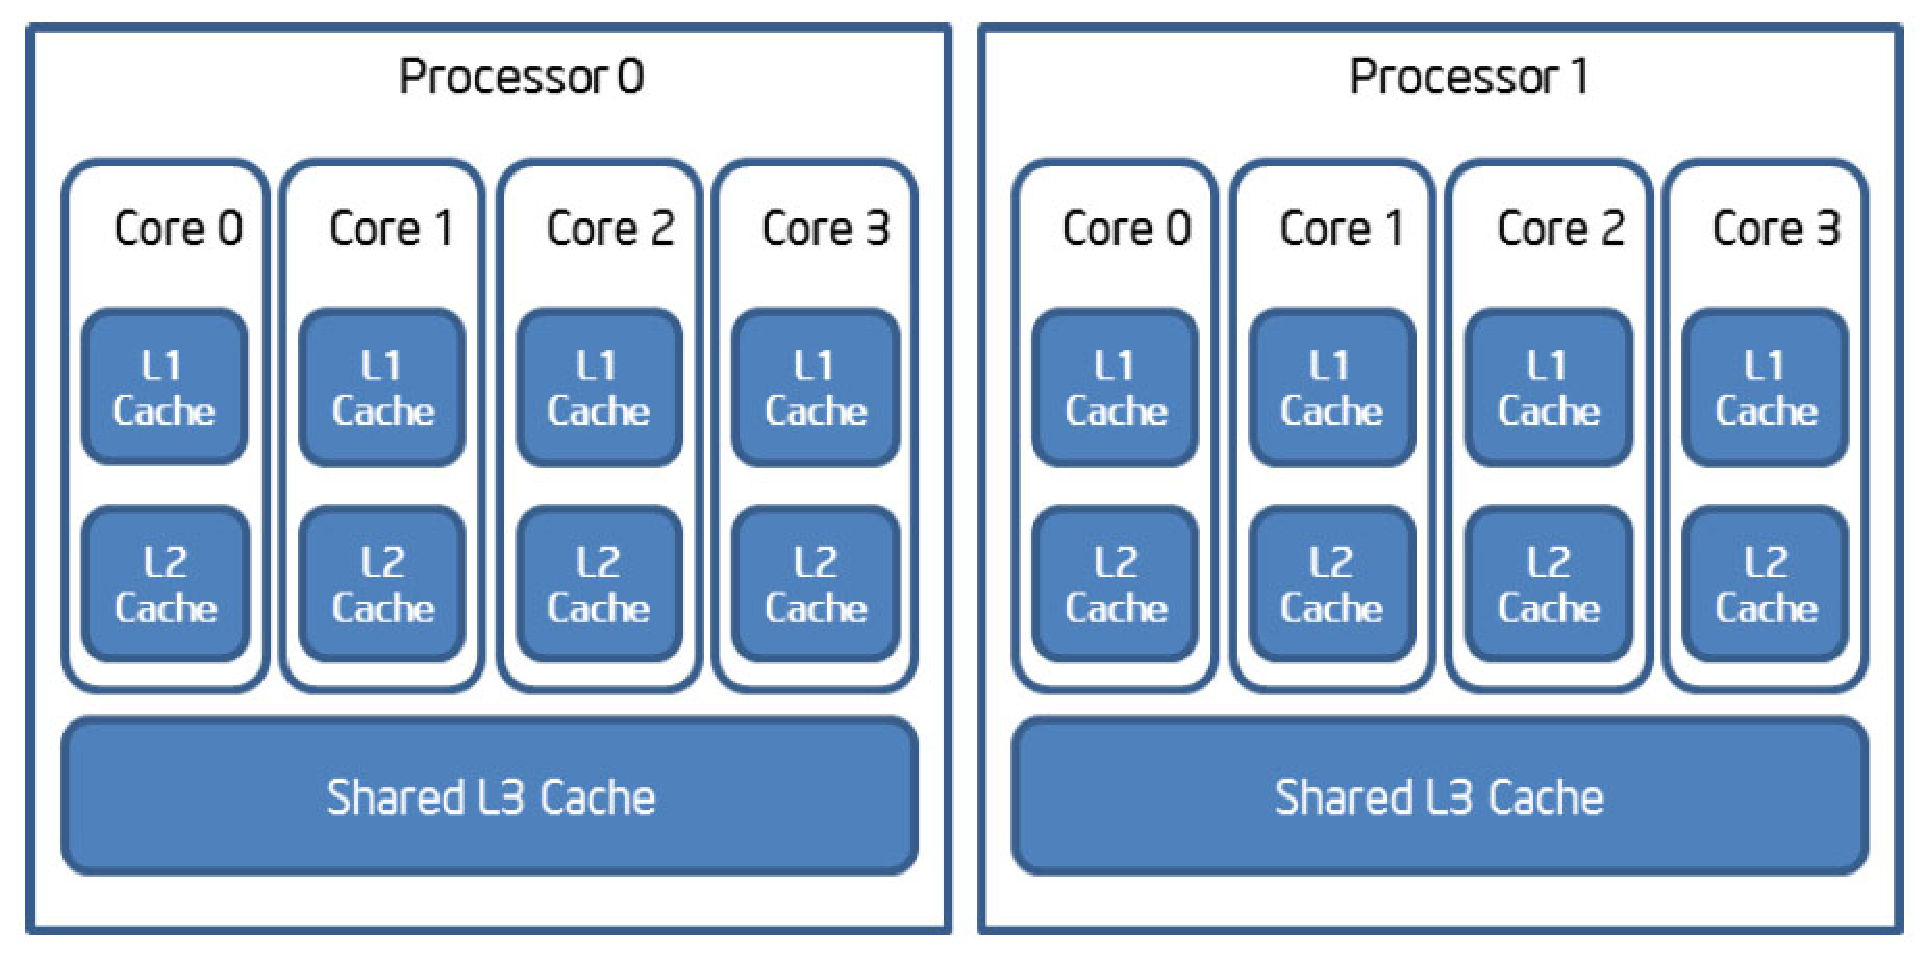
\includegraphics[height=4cm]{./eps/ExampleArchitecture_A.eps}
 \caption{Architecure used in the example}}
 \label{fig:AppAArch}
\end{figurehere}

\begin{tablehere}
{\footnotesize
����\begin{tabular}{|p{8cm}|p{3cm}|p{5cm}|}\hline
Property List&Description&Result on the Example Target Machine\\ \hline
{ CL\_DEVICE\_PARTITION\_EQUALLY, 8, 0 }&
Partition the device into as many sub-devices as possible, each with 8 compute units.&
2 sub-devices, each with 8 threads.\\ \hline
{ CL\_DEVICE\_PARTITION\_EQUALLY, 4, 0 }&
Partition the device into as many sub-devices as possible, each with 4 compute units.&
4 sub-devices, each with 4 threads.\\ \hline
{ CL\_DEVICE\_PARTITION\_EQUALLY, 32, 0 }&
Partition the device into as many sub-devices as possible, each with 32 compute units.&
Error! 32 exceeds the CL\_DEVICE\_PARTITION\_MAX\_ COMPUTE\_UNITS.\\ \hline
{ CL\_DEVICE\_PARTITION\_BY\_COUNTS, 3, 1, CL\_DEVICE\_PARTITION\_BY\_COUNTS\_LIST\_END, 0 }&
Partition the device into two sub-devices, one with 3 compute units and one with 1 compute unit.&
1 sub-device with 3 threads and 1 sub-device with 1 thread.\\ \hline
{ CL\_DEVICE\_PARTITION\_BY\_COUNTS, 2, 2, 2, 2 CL\_DEVICE\_PARTITION\_BY\_COUNTS\_LIST\_END, 0 }&
Partition the device into four sub-devices, each with 2 compute units.&
4 sub-devices, each with 2 threads.\\ \hline
{ CL\_DEVICE\_PARTITION\_BY\_COUNTS, 3, 1, CL\_DEVICE\_PARTITION\_BY\_COUNTS\_LIST\_END, 0 }&
Partition the device into two sub-devices, one with 3 compute units and one with 1 compute unit.&
1 sub-device with 3 threads and 1 sub-device with 1 threads.\\ \hline
{ CL\_DEVICE\_PARTITION\_BY\_AFFINITY\_DOMAIN,
CL\_DEVICE\_AFFINITY\_DOMAIN\_NUMA,
0 }&
Partition the device into sub-devices that share a NUMA node.&
2 sub-devices with 8 threads each. Each sub-device is located on its own NUMA node.\\ \hline
{ CL\_DEVICE\_PARTITION\_BY\_AFFINITY\_DOMAIN,
CL\_DEVICE\_AFFINITY\_DOMAIN\_L1\_CACHE,
0 }&
Partition the device into sub-devices that share an L1 cache.&
8 sub-devices with 2 threads each. The L1 cache is not shared in our example machine.\\ \hline
{ CL\_DEVICE\_PARTITION\_BY\_AFFINITY\_DOMAIN,
CL\_DEVICE\_AFFINITY\_DOMAIN\_L2\_CACHE,
0 }&
Partition the device into sub-devices that share an L2 cache.&
8 sub-devices with 2 thread each. The L2 cache is not shared in our example machine.\\ \hline
{ CL\_DEVICE\_PARTITION\_BY\_AFFINITY\_DOMAIN,
CL\_DEVICE\_AFFINITY\_DOMAIN\_L3\_CACHE,
0 }&
Partition the device into sub-devices that share an L3 cache.&
2 sub-devices with 8 threads each. The L3 cache is shared among all 8 threads within each processor.\\ \hline
{ CL\_DEVICE\_PARTITION\_BY\_AFFINITY\_DOMAIN,
CL\_DEVICE\_AFFINITY\_DOMAIN\_L4\_CACHE,
0 }&
Partition the device into sub-devices that share an L4 cache.&
Error! There is no L4 cache.\\ \hline
{ CL\_DEVICE\_PARTITION\_BY\_AFFINITY\_DOMAIN,
CL\_DEVICE\_AFFINITY\_DOMAIN\_NEXT\_PARTITIONABLE,
0 }&
Partition the device based on the next partitionable domain. In this case, it is NUMA.&
2 sub-devices with 8 threads each. Each sub-device is located on its own NUMA node.\\ \hline
����\end{tabular}}
\caption{Device Partitioning Examples (Source: \textit{OpenCL Device Fission for CPU Performance, Intel Corporation})}
	\label{tab:AppAExample}
\end{tablehere}

\begin{multicols}{2}

%%%%%%%%%%%%%%%%%%%%%%%%%%%%%%%%%%%%%%%%%%%%%%%%%%%%%%%%%%%%%%%%%%%%%%%%%%%%%

% We suggest the use of JabRef for editing your bibliography file (Report.bib)
\bibliographystyle{splncs}
\bibliography{Report}

\end{multicols}
\end{document}
